\chapter{Experiment}
\label{ch:Experiment}
The experiment was conducted on the Raspberry Pi 4 Model B. 
The Pi's computational capabilities are powered by a Broadcom BCM2711 chip \cite{bcm2711-arm}
consisting of four Cortex-A72 processing cores, each having a 48 kB and 32 kB L1 instruction 
and data cache, respectively. The local caches are connected to a central 1 MB L2 cache, which is also 
used by an integrated VideoCore 6 GPU. The SoC interfaces with an 8 GB LPDDR4-SDRAM chip through a 
32-bit wide bus. Hence, two fetch operations are required to load a 64-bit value from memory into 
one of the cores' registers.
A 64 GB SanDisk UHS-1 microSD card is used for persistent storage. The card is connected 
to the SoC through an SDIO interface. For networking, the board comes with an ethernet port and a 
wireless networking module that is connected through an SDIO interface.

A Fedora 36 server image \cite{fedora-36-server} with the 5.17.5 Linux kernel version was flashed 
on the microSD card and installed on the Raspberry Pi. The disk partitions were resized to fully 
incorporate the available disk space, ending up with 56 GB of disk space allocated to the logical volume 
mounted at the root point and 7 GB of swap space. The filesystem mounted at the root point is \verb|xfs|. 
The device was connected to a hidden local WiFi network through the \verb|nmcli| tool. The 
ethernet port remained unused. 

The device was 
put in an aluminium case that acts as a heat-sink and dissipates the heat out of the processor. 
In other words, the case acts as a passive cooling component that protects against potential
performance perturbations caused by thermal trottling. 

Each of the following sections introduces a question equivalent to a performance problem 
statement and a hypothesis that tries to answer it. The hypothesis is proven or disproven based on observational data 
gathered by running the workloads. The data is then analysed. The operational flow is similar for all 
hypotheses. Observational data is gathered by executing the same workload within and outside 
the container abstraction. The differences in the data points act as a proxy metric for the 
isolation overhead of a container. 


\section{Problem A}

\subsection{Problem statement}

In order to properly isolate the container's root filesystem from the host, the runtime 
creates a dedicated mount point that binds the directory on the host to a mount point 
in the container. The mount point has two important properties. First, it is invisible from the host. 
Second, it atomically replaces the root mount within the mount namespace 
of the container. Given this configuration, we can derive the following question:

\textit{Does reading/writing data from the underlying device through a bind mounted root filesystem in 
an isolated mount namespace cause an increase in latency or a decrease in throughput?}

\subsection{Hypothesis}
The two potential sources of isolation overhead are the indirection introduced by the mount namespace 
and the bind mount. 

Examining the source code of the \verb|read()| and \verb|write()| system calls 
shows that the namespace abstraction is used once - to check if the calling process 
has the necessary permissions to operate on the file.
This is done by checking if there is a valid user identifier 
mapping between the user namespace of the calling process and the owning user namespace of the 
file. Both are accessed in constant time - by following pointers relative to the currently 
executing process and the inode that is translated from the file descriptor, respectively.
The inode user identifier is translated into a user identifier within the user namespace 
of the mount namespace where the inode was found.
This is also a constant operation, because identifiers in different user namespaces are mapped using simple 
addition and subtraction \cite{idmappings}.
The translated user identifier is compared
to the user identifier of the current process and if they match, the read operation 
is delegated to the underlying fileystem implementation - \verb|xfs|. If the identifiers do not match, 
the access control lists of the inode are consulted before delegating. 
The ACL subsystem asseses the permissions of the process through a multitude of bitwise operations, which 
are also constant. 

Setting up the bind mount should not have an effect on these system calls. The overhead of that operation manifests itself
during the container creation phase - when a duplicate view of the directory holding 
the container's root filesystem is created under a new node in the file system hierarchy.

The argumentation above leads to the following hypothesis:

\textit{Reading and writing data from a device through a bind mounted root filesystem resident in an isolated mount namespace exhibits
the same latency and throughput characteristics as performing the equivalent operationse in the root mount namespace without a bind mount.}

\subsection{Test}
In order to test the hypothesis, the filesystem workload ran for both the read and write 
operations within and outside a container. The workload's total runtime was 60 seconds.
No concurrent operations were executed - a single process issued a single operation per unit of time. 
During the workload's runtime, the number of successfully executed input-output operations and the total latency per second 
were accumulated. The results for the read and write system calls are shown in Figure \ref{ch:experiment/problem-a/test/read-iops-over-time},
Figure \ref{ch:experiment/problem-a/test/write-iops-over-time}, Figure \ref{ch:experiment/problem-a/test/read-latency-over-time} and Figure \ref{ch:experiment/problem-a/test/write-latency-over-time}.

\begin{figure}[H]
    \centering
    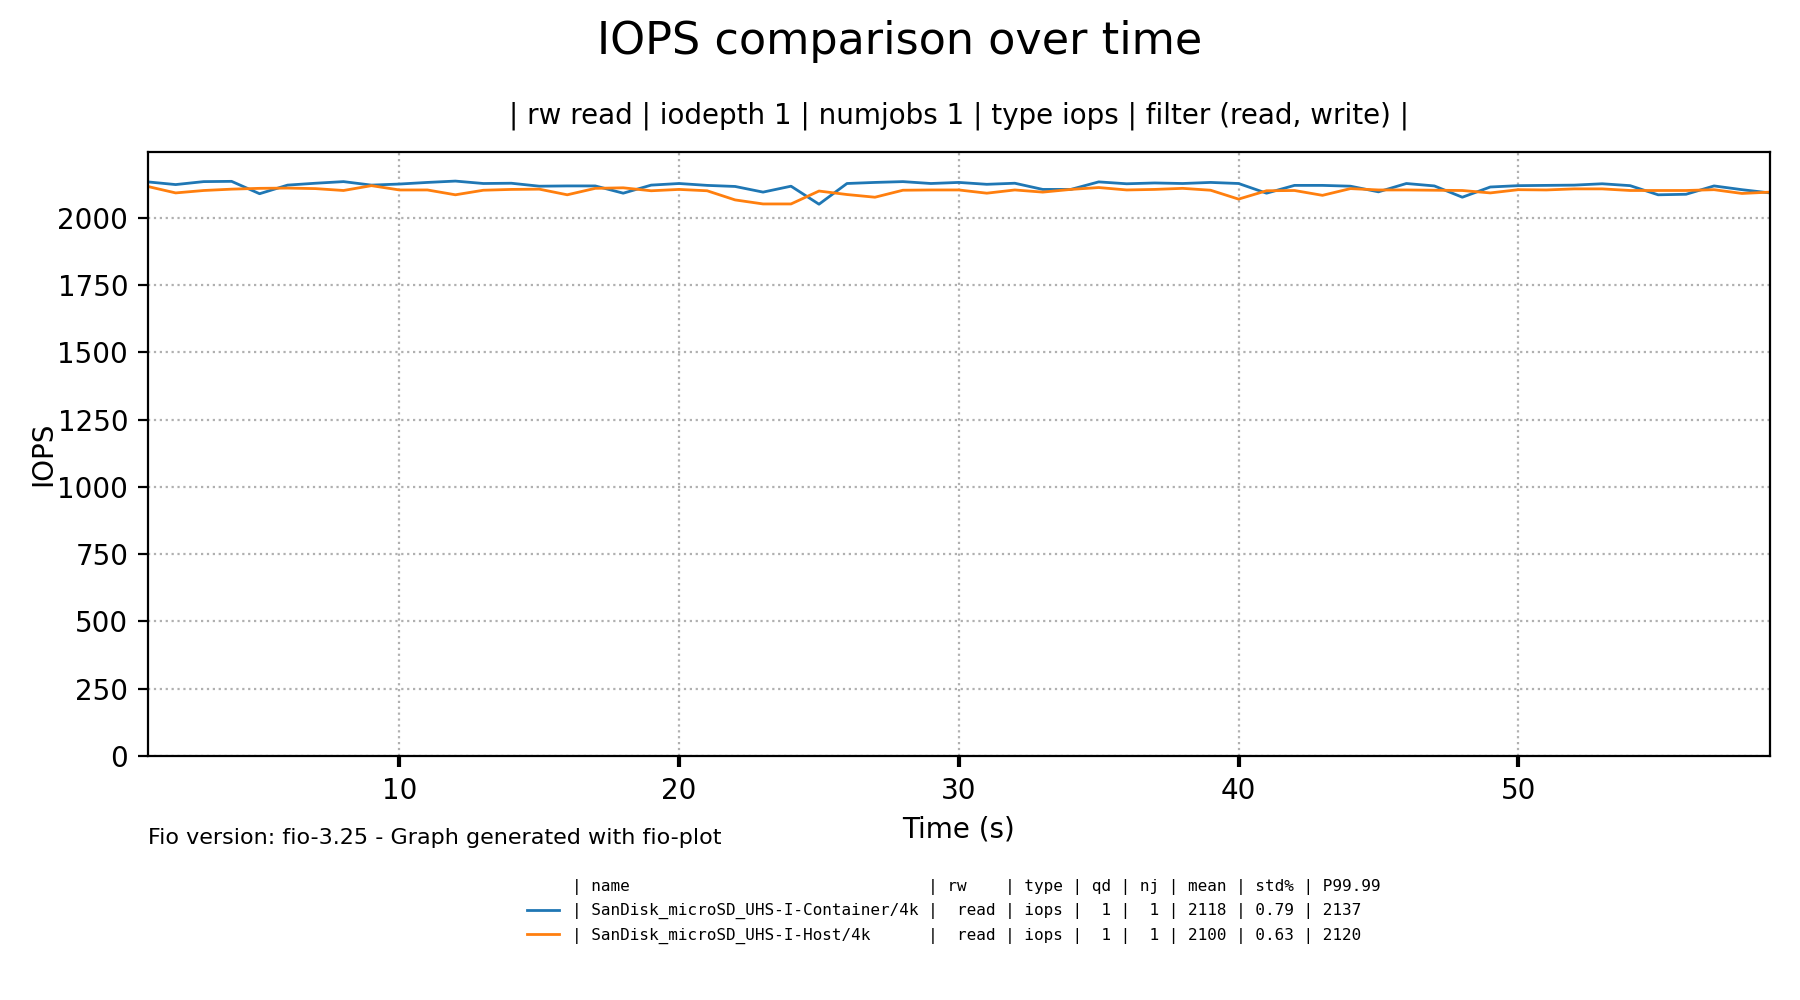
\includegraphics[width=0.8\textwidth]{images/results/sandisk-libaio-iops-read-comparison.png}
    \caption{Read IOPS on the host and inside a container, compared over time}
    \label{ch:experiment/problem-a/test/read-iops-over-time}
\end{figure}
\begin{figure}[H]
    \centering
    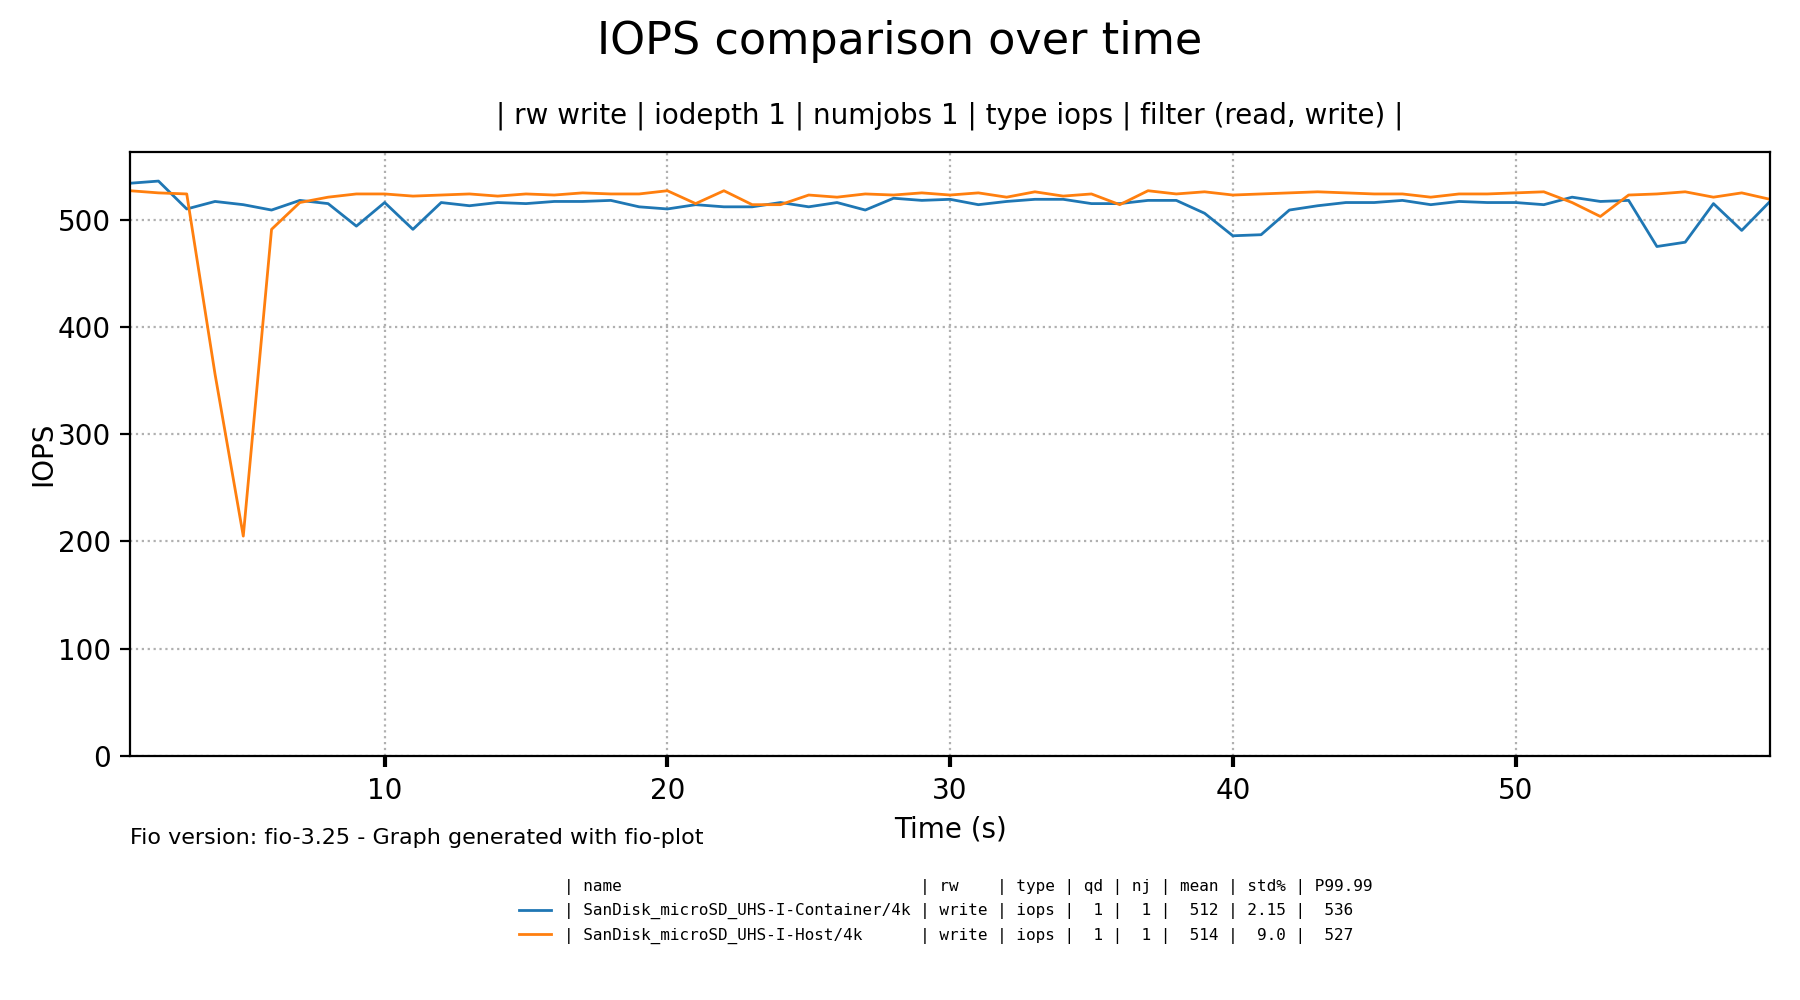
\includegraphics[width=0.8\textwidth]{images/results/sandisk-libaio-iops-write-comparison-2.png}
    \caption{Write IOPS on the host and inside a container, compared over time}
    \label{ch:experiment/problem-a/test/write-iops-over-time}
\end{figure}

\begin{figure}[H]
    \centering
    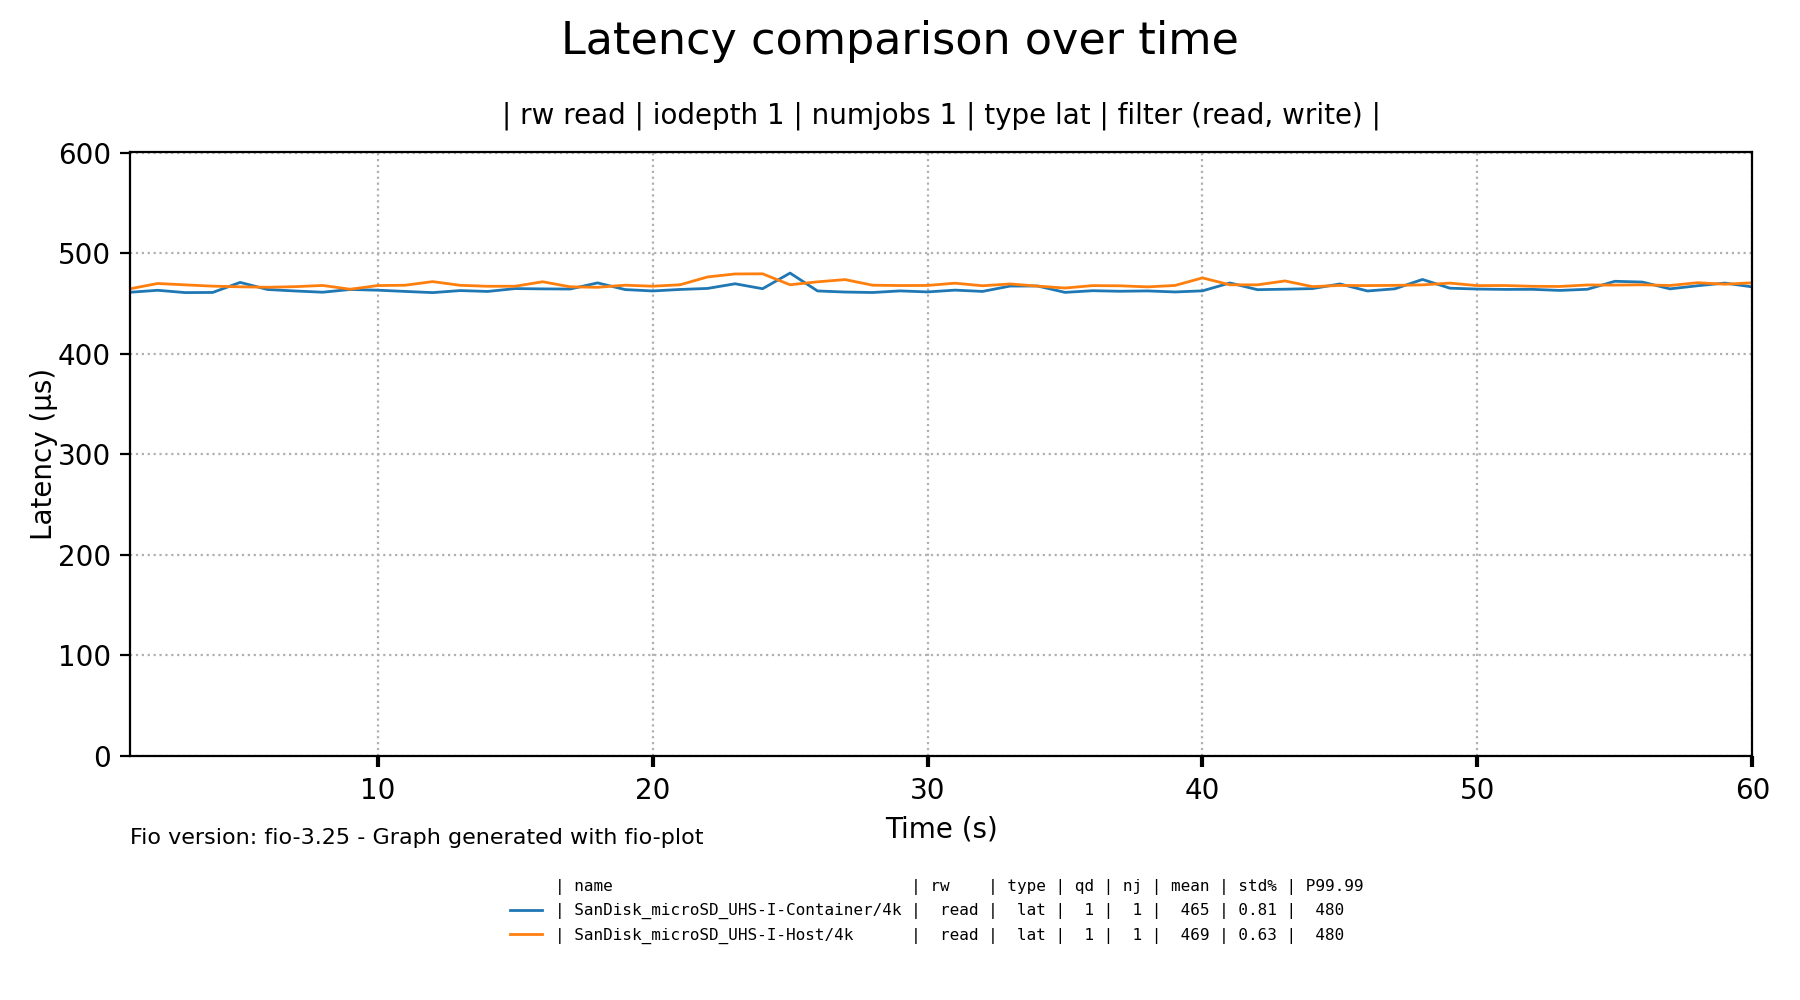
\includegraphics[width=0.8\textwidth]{images/results/sandisk-libaio-latency-read-comparison.png}
    \caption{Read latency on the host and inside a container, compared over time}
    \label{ch:experiment/problem-a/test/read-latency-over-time}
\end{figure}
\begin{figure}[H]
    \centering
    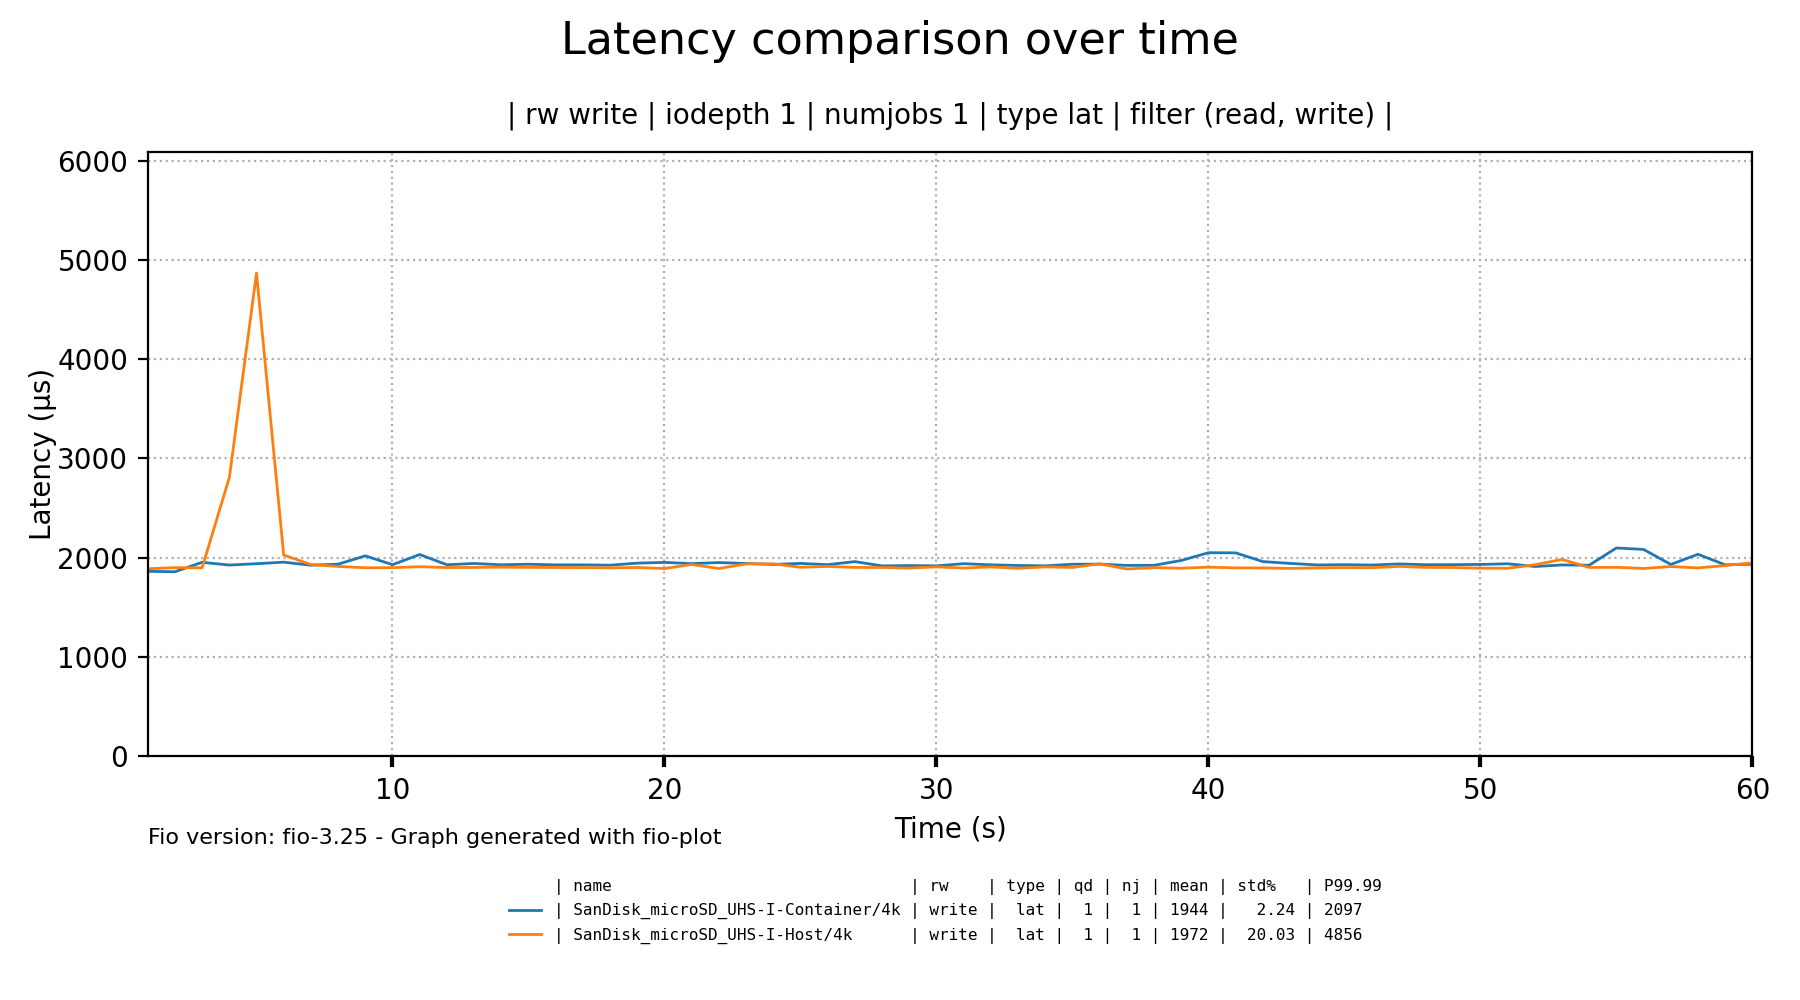
\includegraphics[width=0.8\textwidth]{images/results/sandisk-libaio-latency-write-comparison-2.png}
    \caption{Write latency on the host and inside a container, compared over time}
    \label{ch:experiment/problem-a/test/write-latency-over-time}
\end{figure}

\subsection{Analysis}
Figure \ref{ch:experiment/problem-a/test/read-iops-over-time} plots the number of read operations per second 
within and outside a container. The orange line denotes the values accumulated on the host, whilst the blue line 
highlights the container's accumulations. The results show that reading data through a bind mounted root filesystem 
within a separate mount namespace has no impact on read throughput. The container handles, on average,
8 more read operations than the host throughout the workload's lifetime. This, however, is arbitrary
and varies across workload runs. As can be seen by the graph, the throughput achieved is nearly 
identical during the entire workload's lifespan.

Figure \ref{ch:experiment/problem-a/test/read-latency-over-time} plots the latency (in microseconds) 
achieved within and outside a container. The graph tells a similar story. Latencies are stable and 
do not deviate by more than $0.81$\% from an average of $0.45$ milliseconds. 

Write operations exhibit higher latencies and lower throughputs.
So much so that the difference in read and write performance is a factor of three.
In addition, write samples deviate a lot more from their mean value compared to 
read samples, as can be seen in Figure \ref{ch:experiment/problem-a/test/write-iops-over-time}
and Figure \ref{ch:experiment/problem-a/test/write-latency-over-time}. The host 
has a significant outlier in the beginning but then achieves better throughput and lower 
latency throughout the end. The container destabilises at the end of the workload.
In the end, however, the mean average IOPS within the container are $512$, whereas on the host 
they are $514$ - a negligible difference. The same can be said for the latency - $1.94$ milliseconds compared to 
$1.97$ milliseconds for the container and the host, respectively.  Hence, the hypothesis remains valid.

\section{Problem B}
\subsection{Problem statement}
Efficiently sharing resources between different processes is one of the primary task of a kernel.
As the number of processes utilising the same resource increases, a point of saturation may be reached. 
This happens when the resource reaches 100\% utilisation and queuing begins to be frequent and significant.
A natural question follows:

\textit{Does scaling the number of reads/writes from/to the underlying device issued from a bind mounted 
root filesystem in an isolated mount namespace saturate the resource faster than performing the 
equivalent scaling without the noninterference boundary?}

This question directly follows the performance axiom in Section \ref{sections:fundamentals/virtualisation/axioms/performance}.
Does the overhead introduced by the container runtime to isolate the filesystem negatively affect 
the ability of processes in the container to share a given resource?

\subsection{Hypothesis}
From the previous problem, we know that the difference in latency and throughput outside 
and within the container's noninterference boundary is negligible and has no statistical significance.
Hence, a single process is not negatively affected. Assuming that scaling the number of reads/writes 
is done by increasing the number of processes that concurrently issue input-output operations, then 
the point of saturation should be exactly the same as on the host.

\subsection{Test}
In order to test the hypothesis, the filesystem workload ran for both the read and write 
operations within and outside a container. The workload's total runtime was 60 seconds.
The number of processes was scaled $n$ times by $2^{i}$ for $i = 0\hdots n$ where $n = 6$. 
During the workload's runtime, the number of successfully executed input-output operations and the total latency per second 
were accumulated per process group. The test results are shown in Figure \ref{images:experiment/sandisk-host-libaio-read-numjobs-iops-latency.png},
Figure \ref{images:experiment/sandisk-libaio-read-numjobs-iops-latency.png}, Figure \ref{images:experiment/sandisk-host-libaio-write-numjobs-iops-latency.png}
and Figure \ref{images:experiment/sandisk-libaio-write-num-jobs-iops-latency.png}.

\begin{figure}[H]
    \centering
    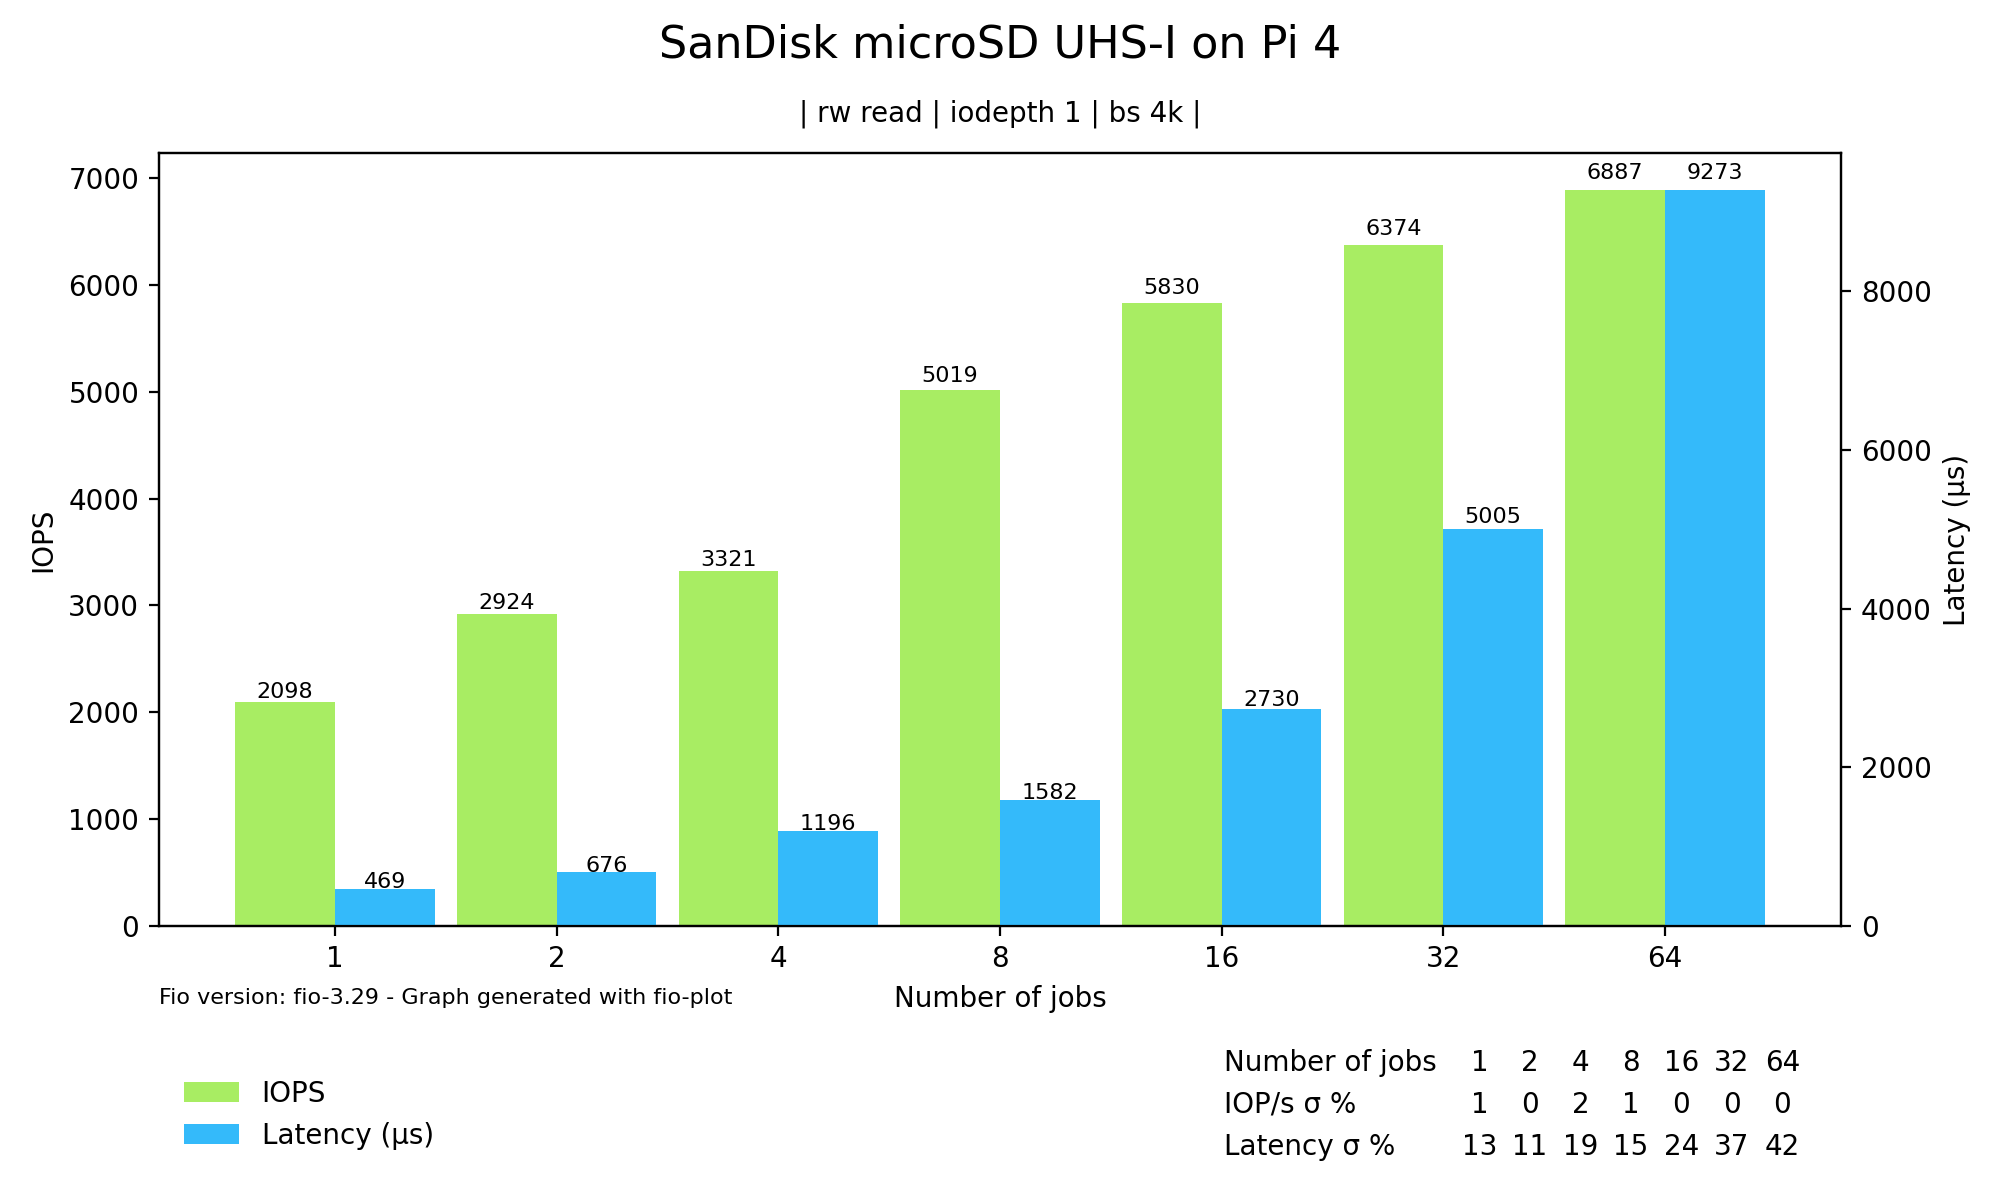
\includegraphics[width=0.7\textwidth]{images/results/sandisk-host-libaio-read-numjobs-iops-latency.png}
    \caption{Throughput and latency measurements on the host as a function of the number of concurrent processes issuing read operations.}
    \label{images:experiment/sandisk-host-libaio-read-numjobs-iops-latency.png}
\end{figure}

\begin{figure}[H]
    \centering
    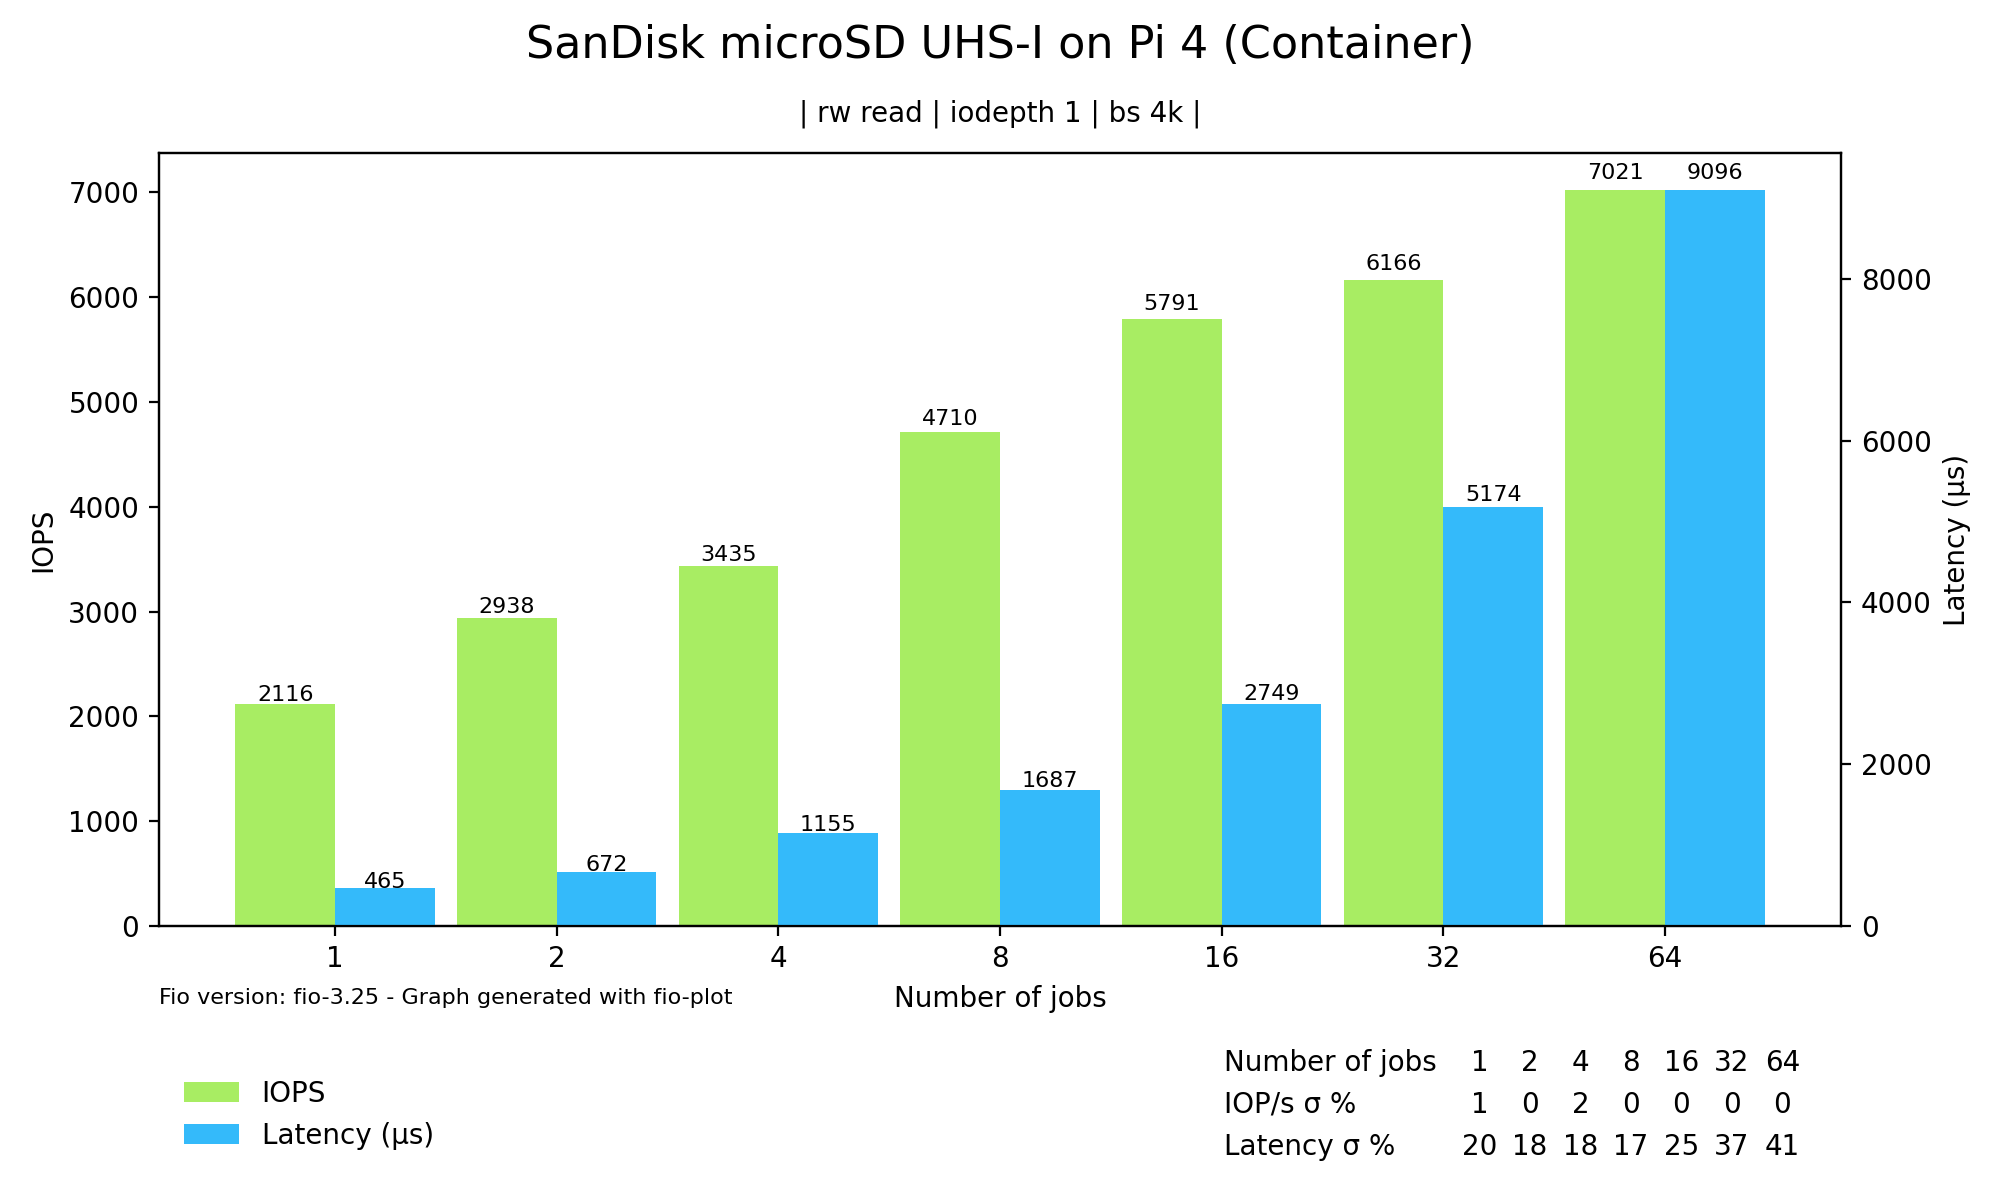
\includegraphics[width=0.7\textwidth]{images/results/sandisk-libaio-read-numjobs-iops-latency.png}
    \caption{Throughput and latency measurements in a container as a function of the number of concurrent processes issuing read operations.}
    \label{images:experiment/sandisk-libaio-read-numjobs-iops-latency.png}
\end{figure}

\begin{figure}[H]
    \centering
    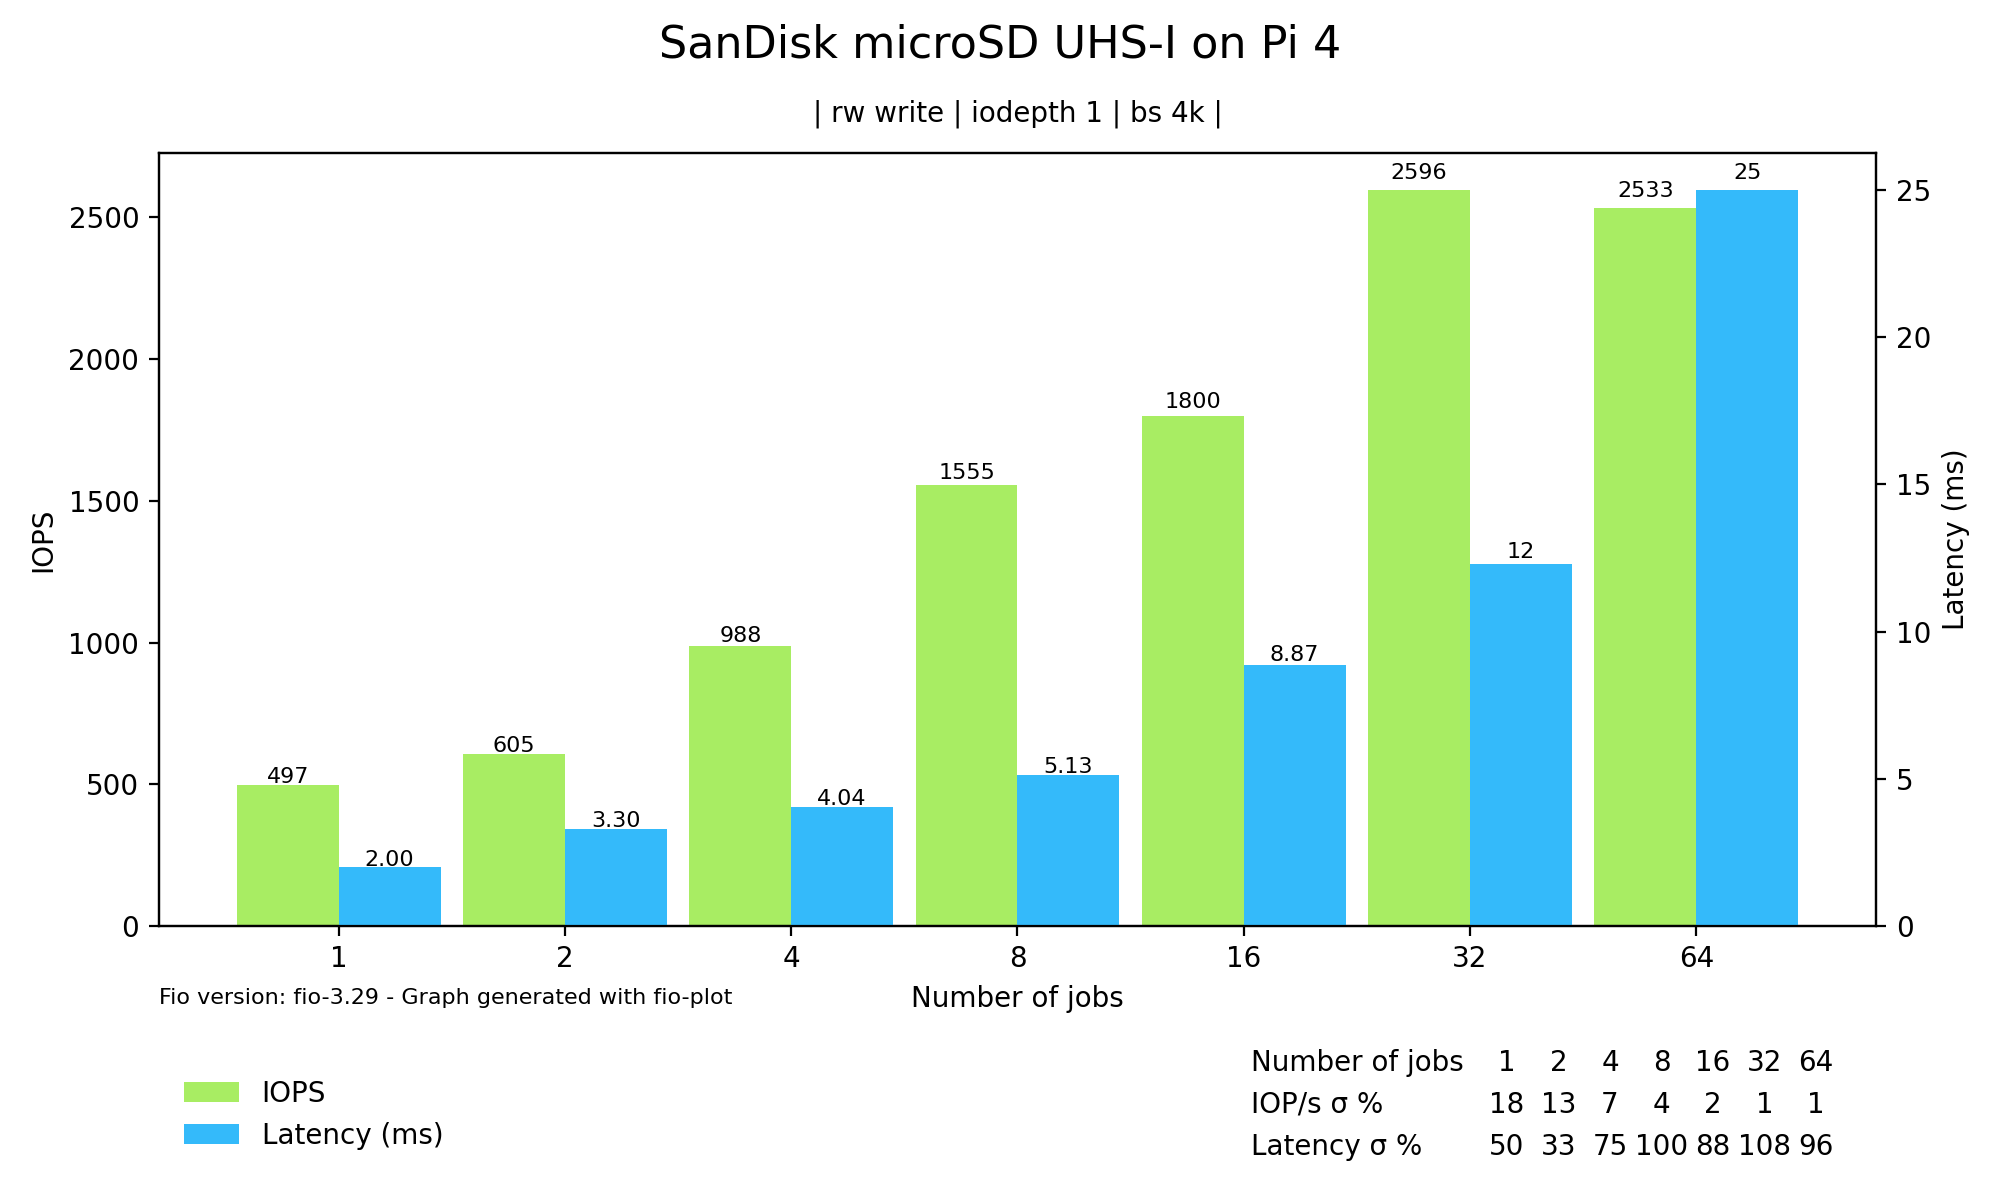
\includegraphics[width=0.7\textwidth]{images/results/sandisk-host-libaio-write-numjobs-iops-latency.png}
    \caption{Throughput and latency measurements on the host as a function of the number of concurrent processes issuing write operations.}
    \label{images:experiment/sandisk-host-libaio-write-numjobs-iops-latency.png}
\end{figure}

\begin{figure}[H]
    \centering
    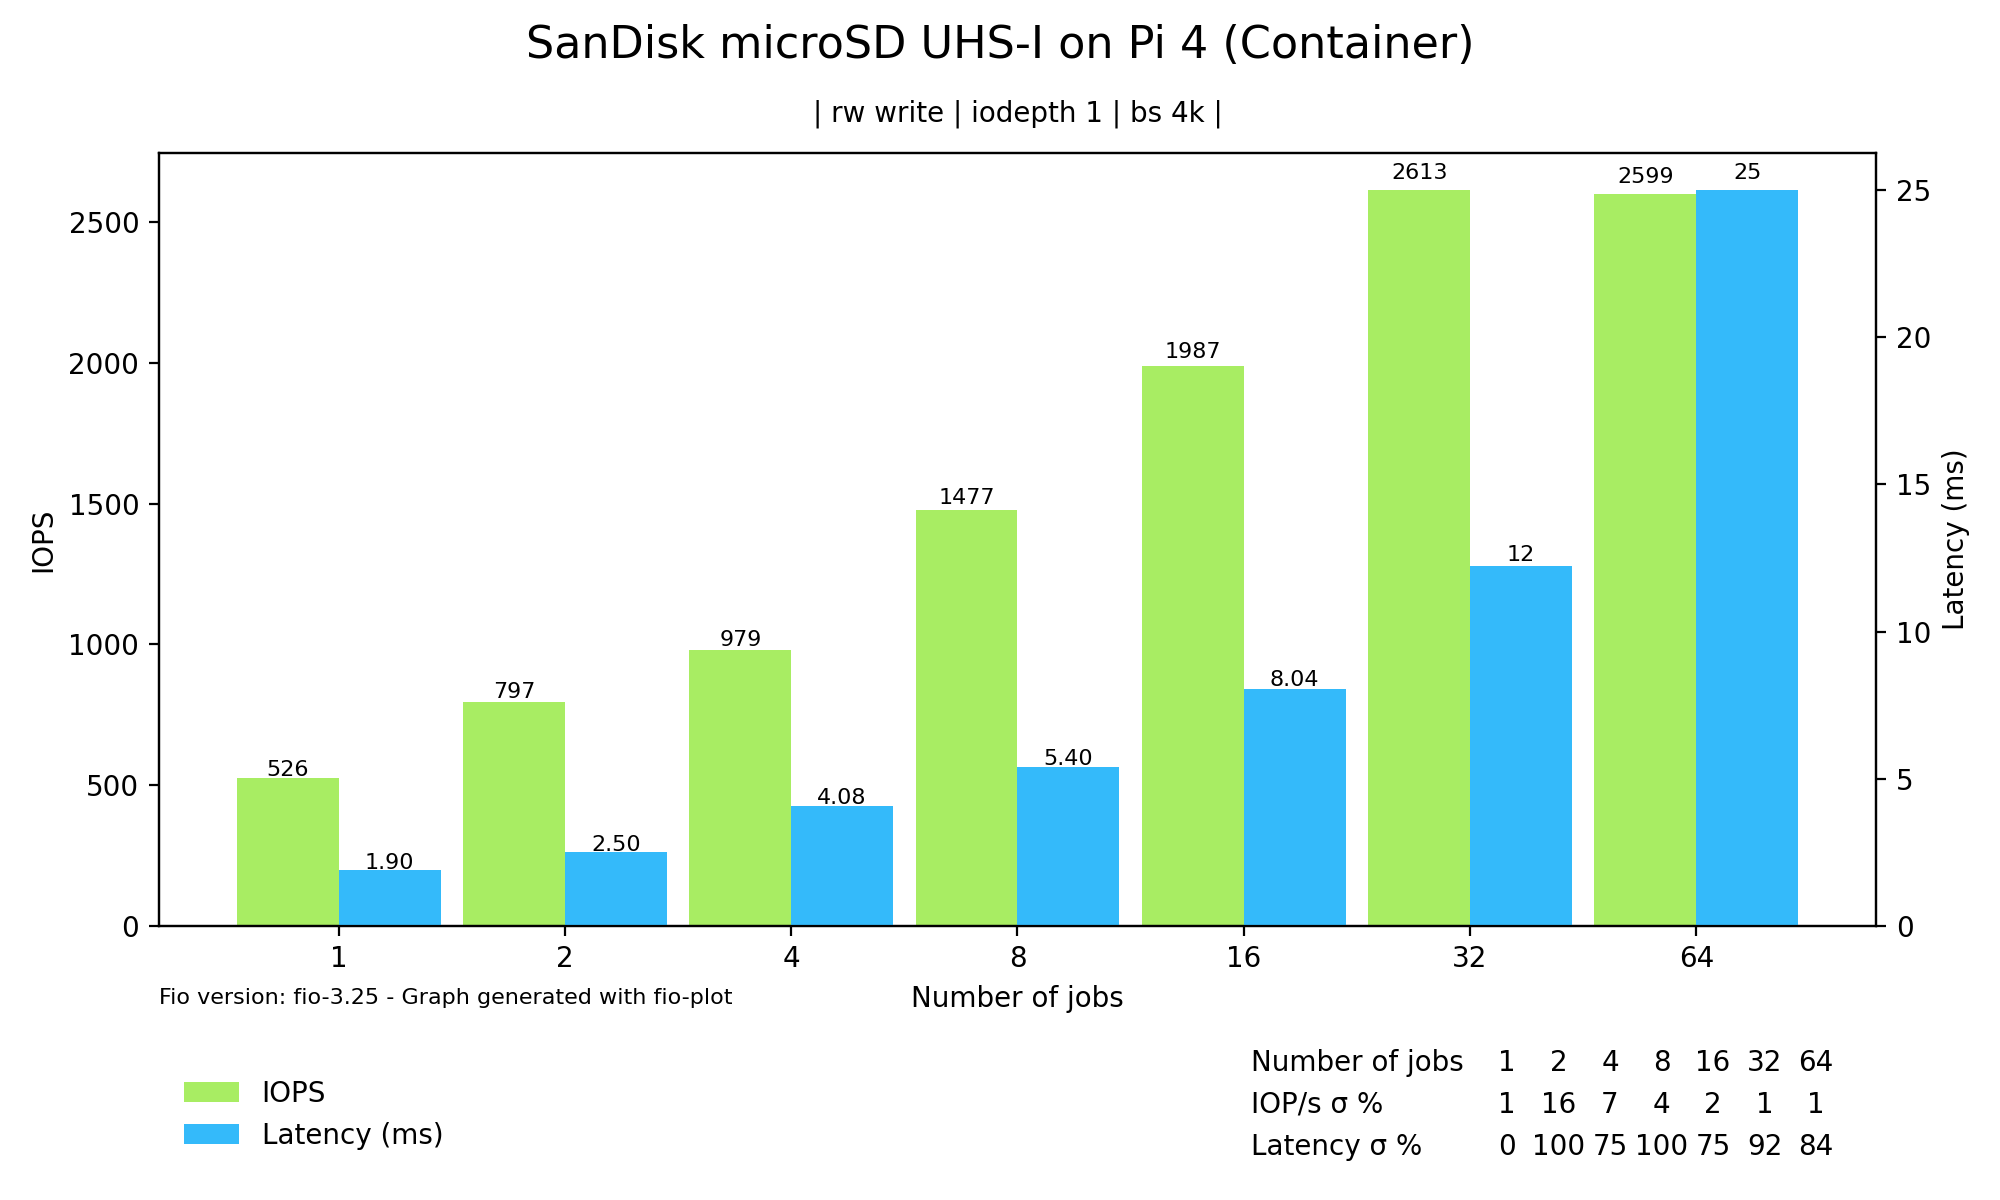
\includegraphics[width=0.7\textwidth]{images/results/sandisk-libaio-write-num-jobs-iops-latency.png}
    \caption{Throughput and latency measurements in a container as a function of the number of concurrent processes issuing write operations.}
    \label{images:experiment/sandisk-libaio-write-num-jobs-iops-latency.png}
\end{figure}

\subsection{Analysis}
Every figure shows the number of concurrent processes issuing the respective operation on the 
x-axis. The y-axis on the left side represents the number of IOPS conducted. The green bars 
show the average number of IOPS achieved during the workload's execution. The y-axis on the right side 
represents the latency (in microseconds) The blue bars show the average latency during the workload's execution. 

Figure \ref{images:experiment/sandisk-host-libaio-read-numjobs-iops-latency.png} and 
Figure \ref{images:experiment/sandisk-libaio-read-numjobs-iops-latency.png} show the 
number of IOPS and the latency for the read operation on the host and in a container, respectively. 
In both cases, the same tendency is observed. As the number of processes is increased, then 
the number of successfully executed input-output operations increases as well.
Similarly, latency increases as well. The best IOPS to latency ratio on the host is observed 
when the number of concurrently running processes is $8$. The point of saturation is reached 
at approximately $32$ concurrent processes where the IOPS to latency ratio is worse then running 
a single process. In the container, the best ratio is observed when the number of concurrent 
processes is $16$. Both the host and the container have the same point of saturation - at 
$32$ processes. Hence, for reads, the hypothesis holds. However, to achieve the best 
resource utilisation, the container needs to create twice as many processes compared to the host - 16 versus 8, respectively. 

% READS: 
% Host: 1629, 2248, 2125, 3437, 3100, 1369, -2386
% Container: 1651, 2266, 2280, 3023, 3042, 992, -2075


\section{Filesystem}
\label{ch:experiment/filesystem}

\begin{figure}[H]
    \centering
    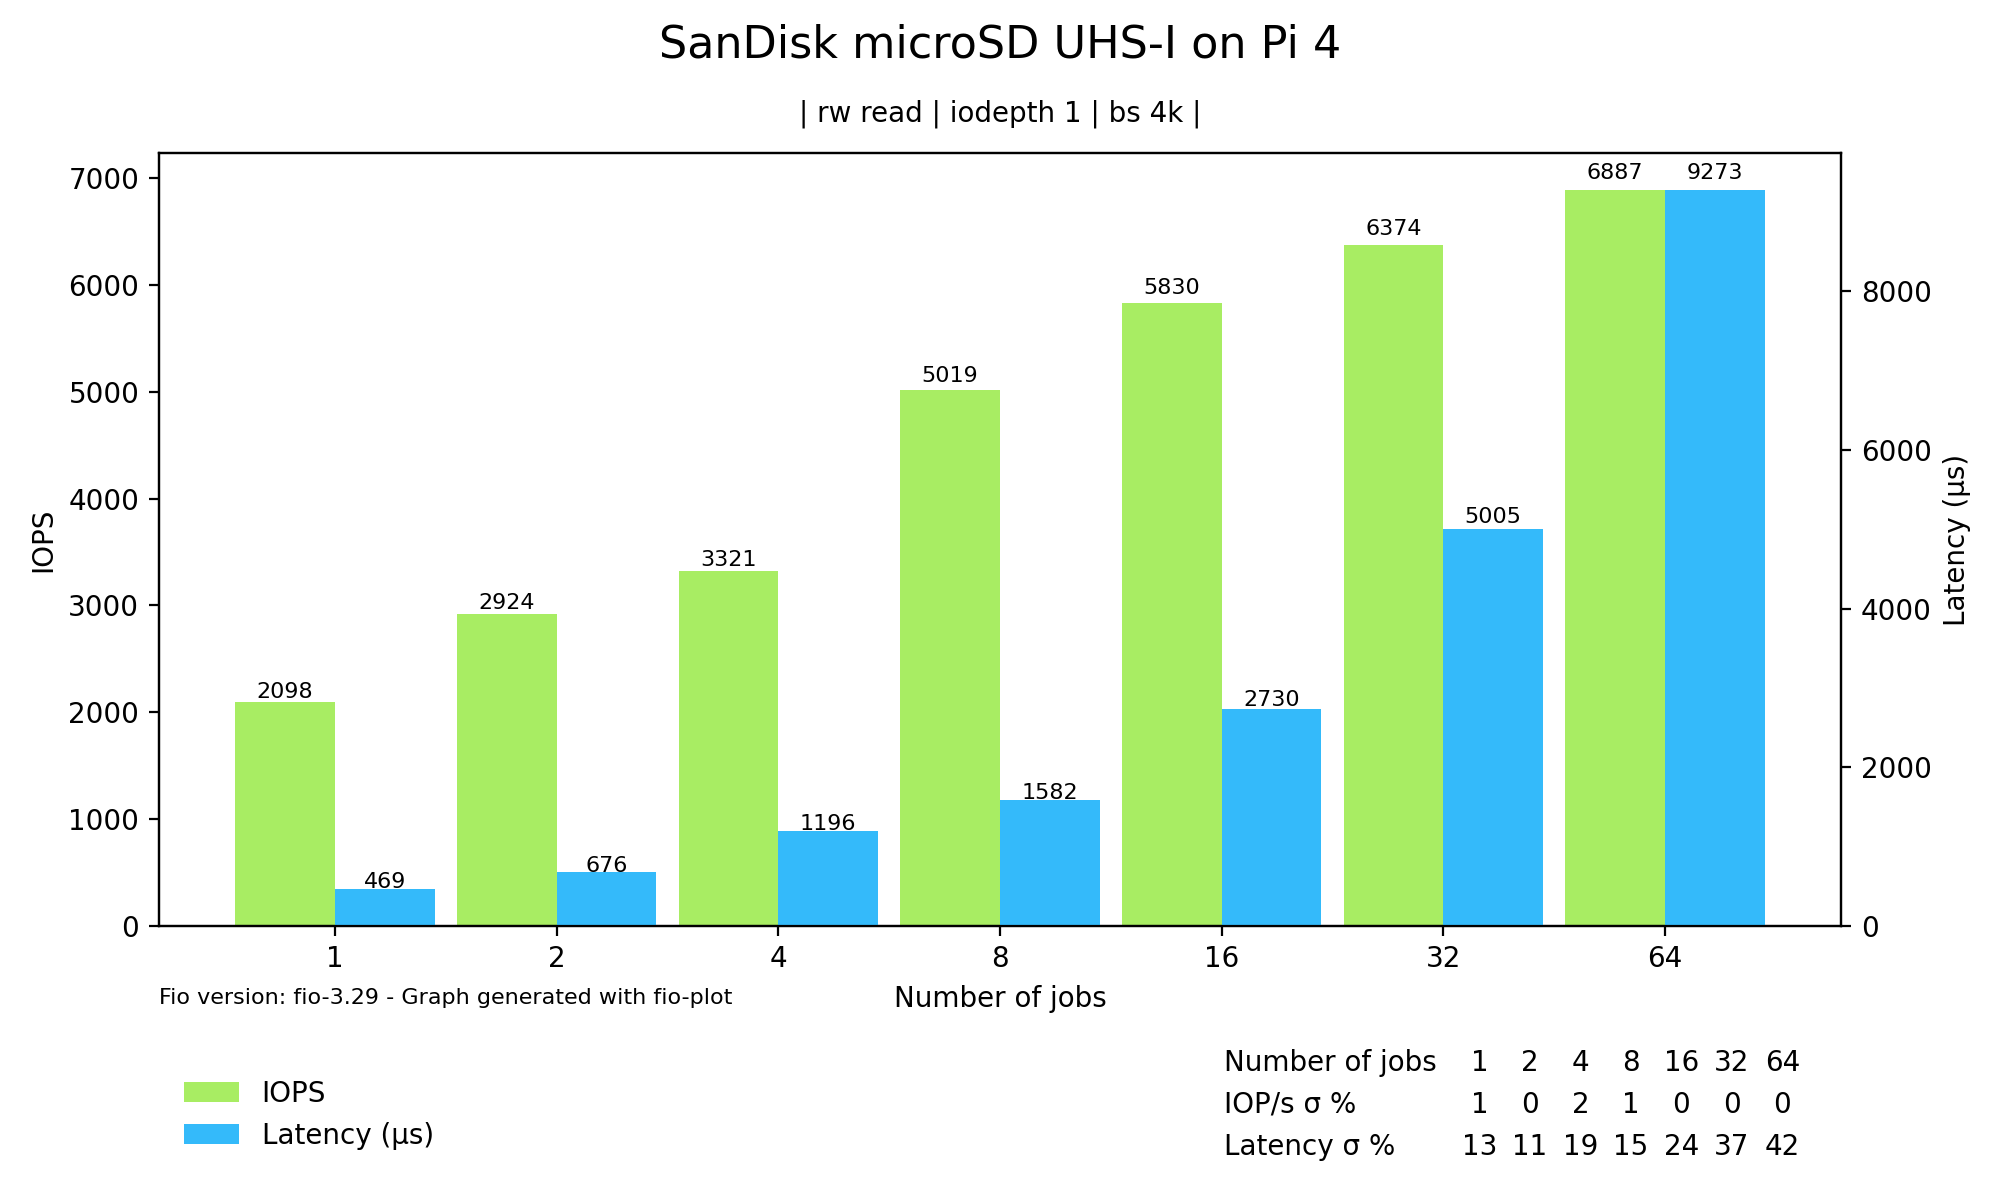
\includegraphics[width=0.8\textwidth]{images/results/sandisk-host-libaio-read-numjobs-iops-latency.png}
    \caption{Throughput and latency measurements on the host as a function of the number of concurrent processes issuing asynchronous reads.}
    \label{images:fundamentals/net-ns-veth-arch.jpg}
\end{figure}

\begin{figure}[H]
    \centering
    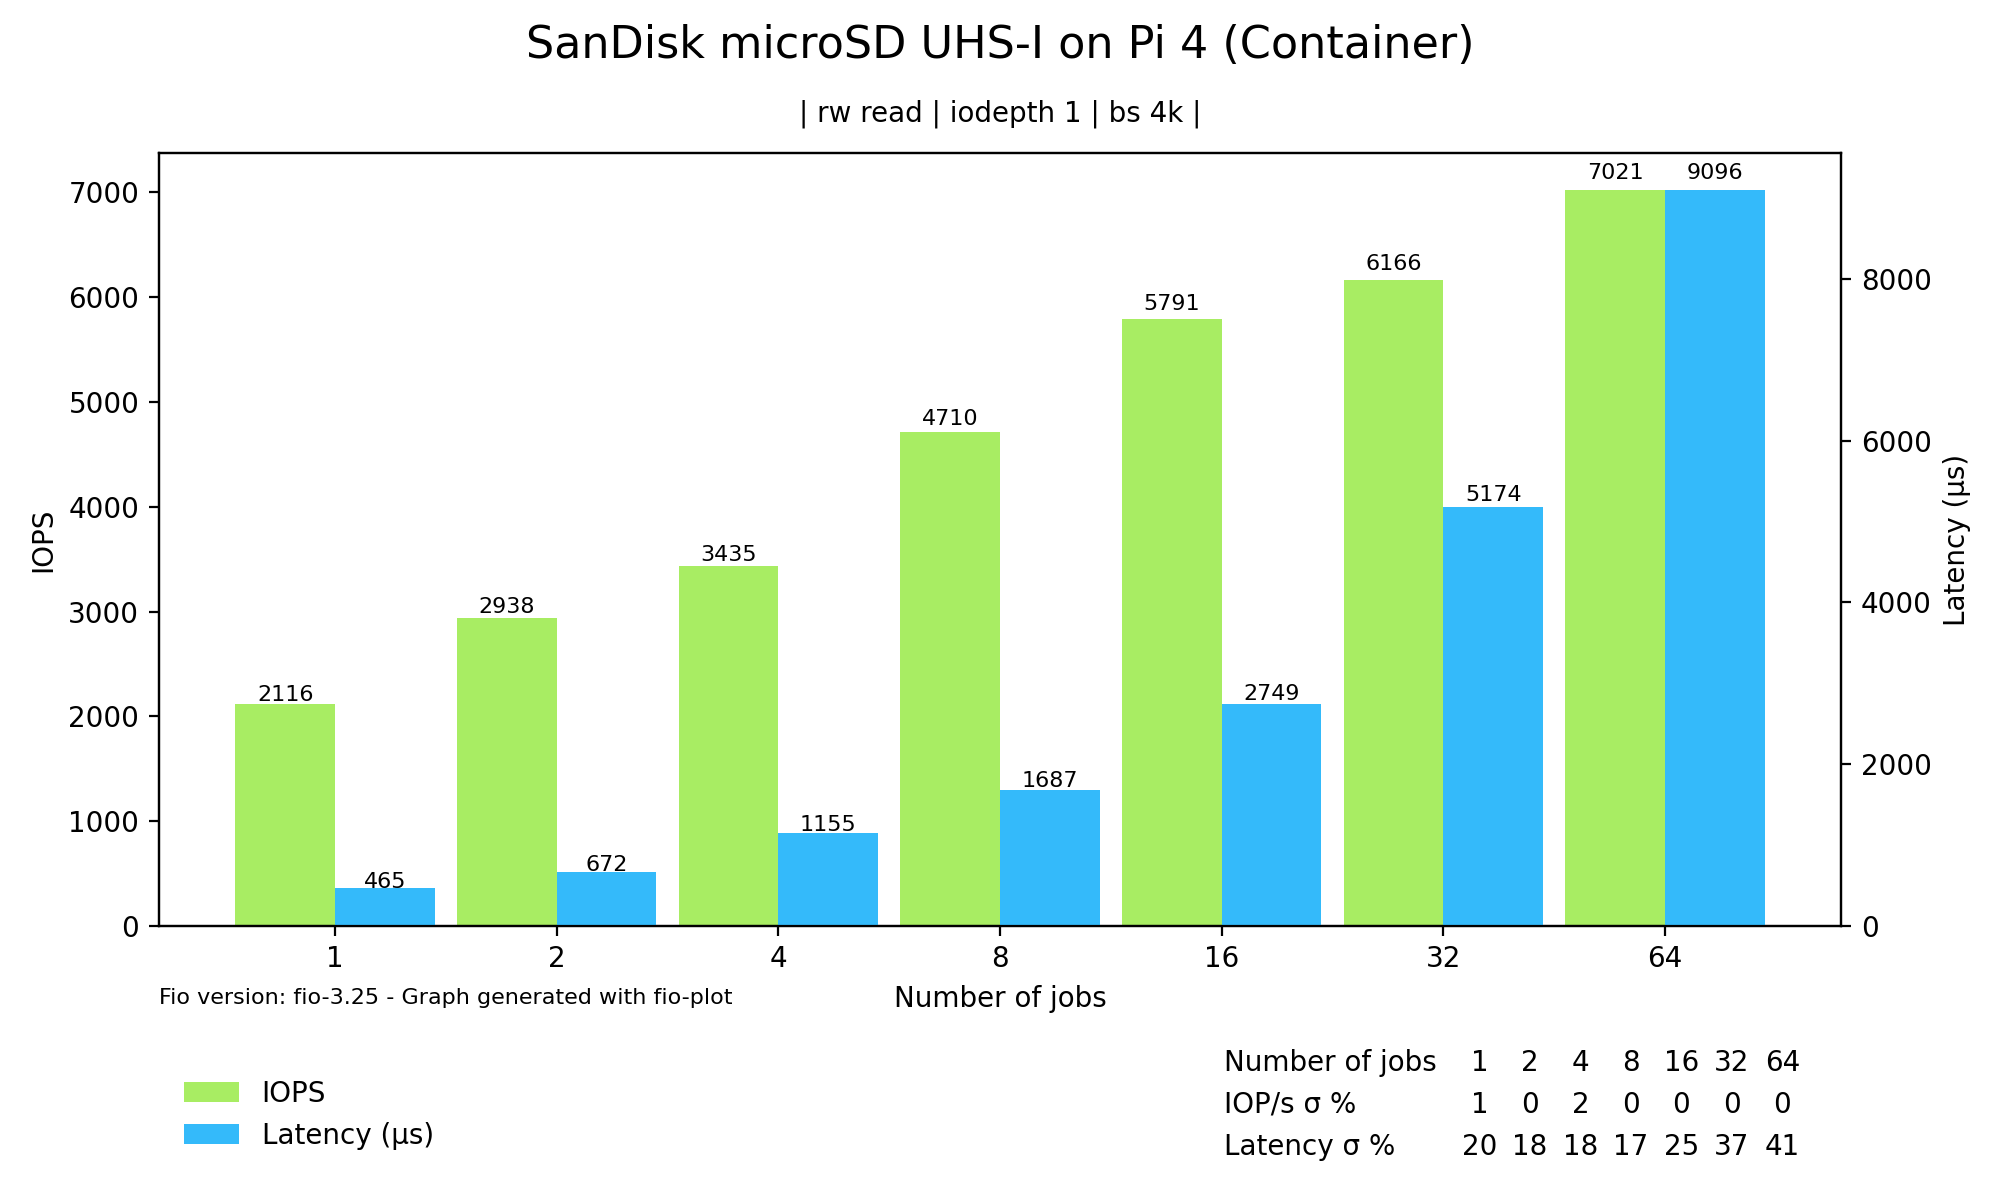
\includegraphics[width=0.8\textwidth]{images/results/sandisk-libaio-read-numjobs-iops-latency.png}
    \caption{Throughput and latency measurements within a container as a function of the number of concurrent processes issuing asynchronous reads.}
    \label{images:fundamentals/net-ns-veth-arch.jpg}
\end{figure}

\begin{figure}[H]
    \centering
    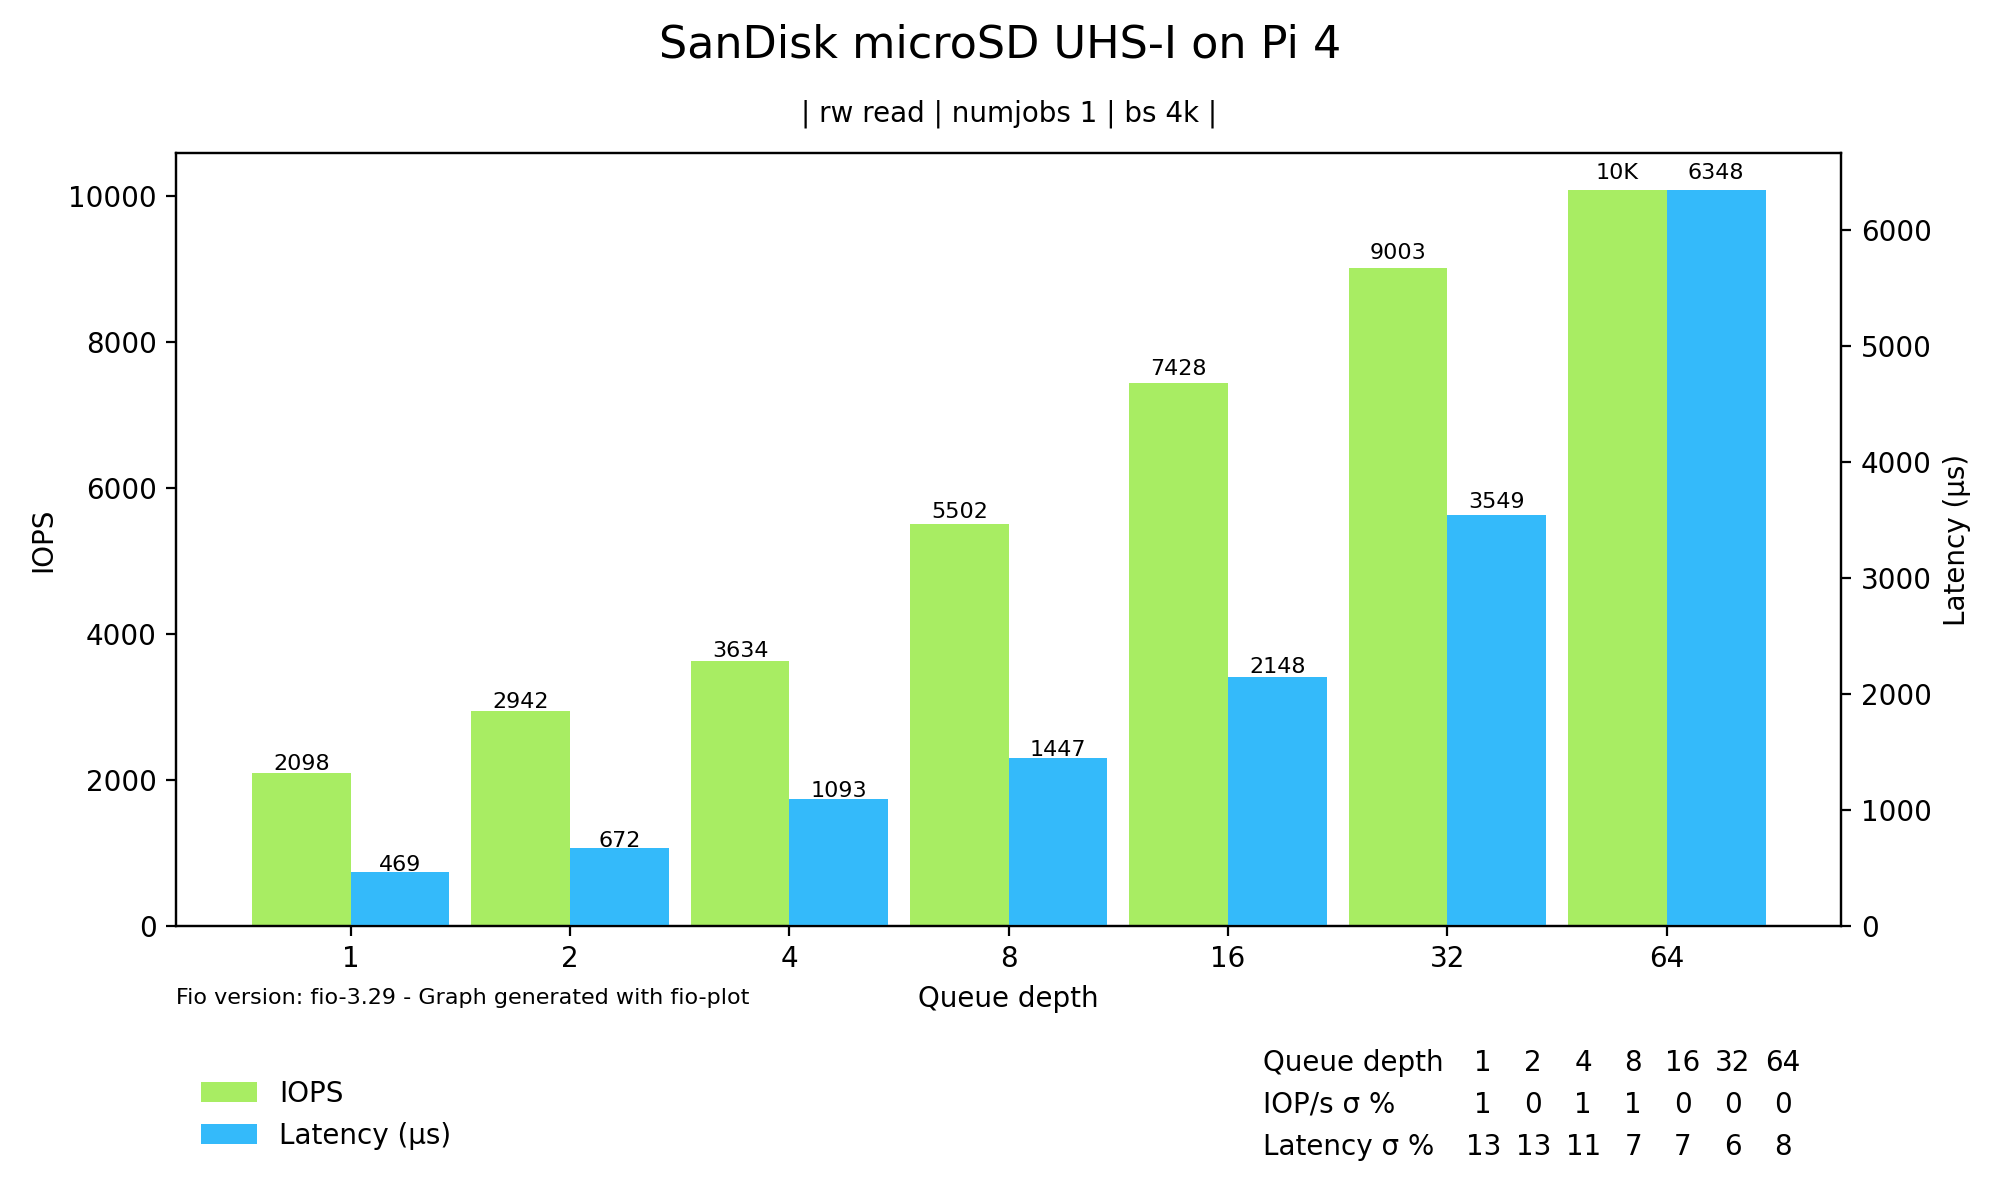
\includegraphics[width=0.8\textwidth]{images/results/sandisk-host-libaio-read-queue-depth-iops-latency.png}
    \caption{Throughput and latency measurements on the host as a function of the transmission queue length holding requests for asynchronous reads.}
    \label{images:fundamentals/net-ns-veth-arch.jpg}
\end{figure}

\begin{figure}[H]
    \centering
    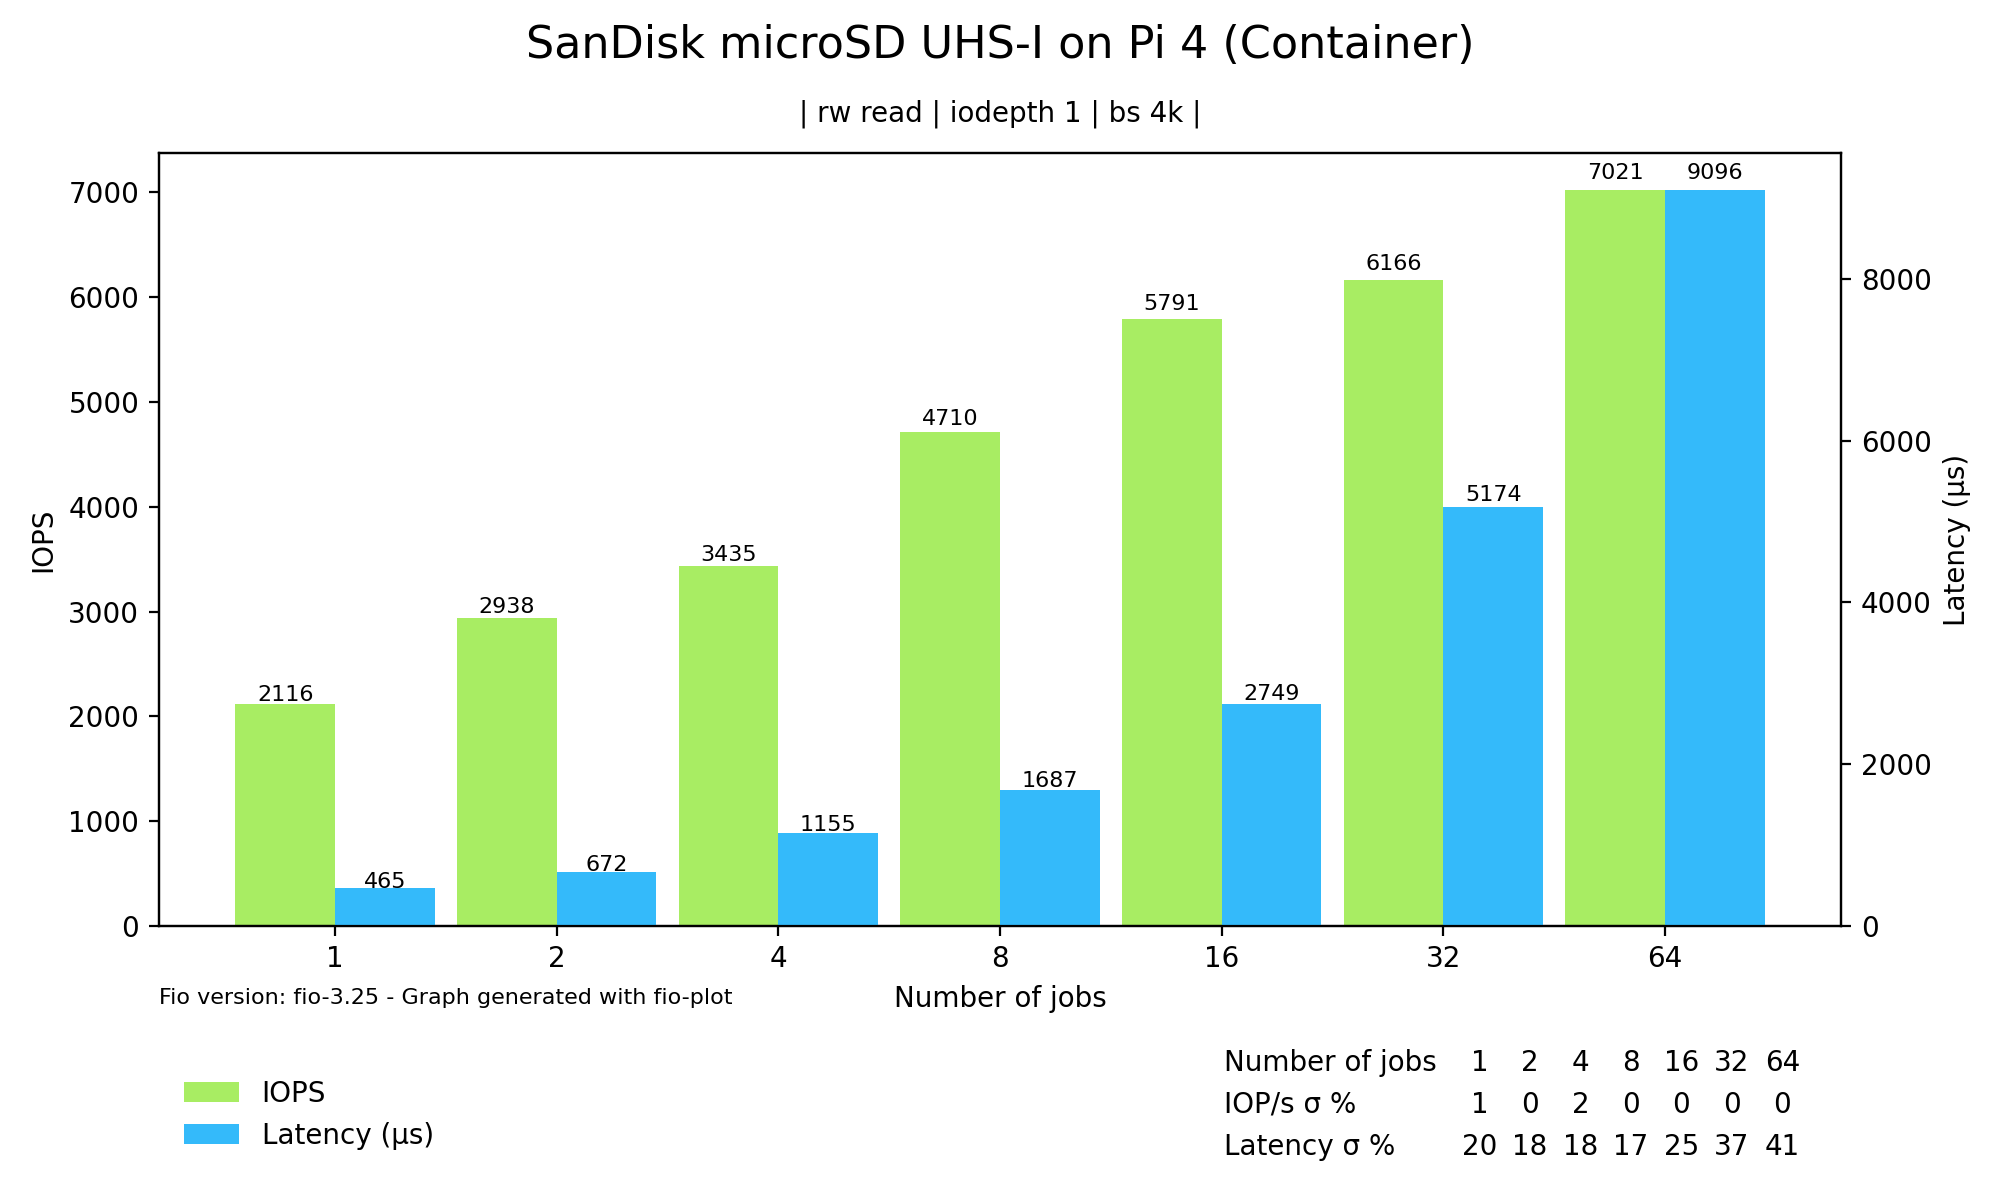
\includegraphics[width=0.8\textwidth]{images/results/sandisk-libaio-read-numjobs-iops-latency.png}
    \caption{Throughput and latency measurements within a container as a function of the transmission queue length holding requests for asynchronous reads.}
    \label{images:fundamentals/net-ns-veth-arch.jpg}
\end{figure}

\begin{figure}[H]
    \centering
    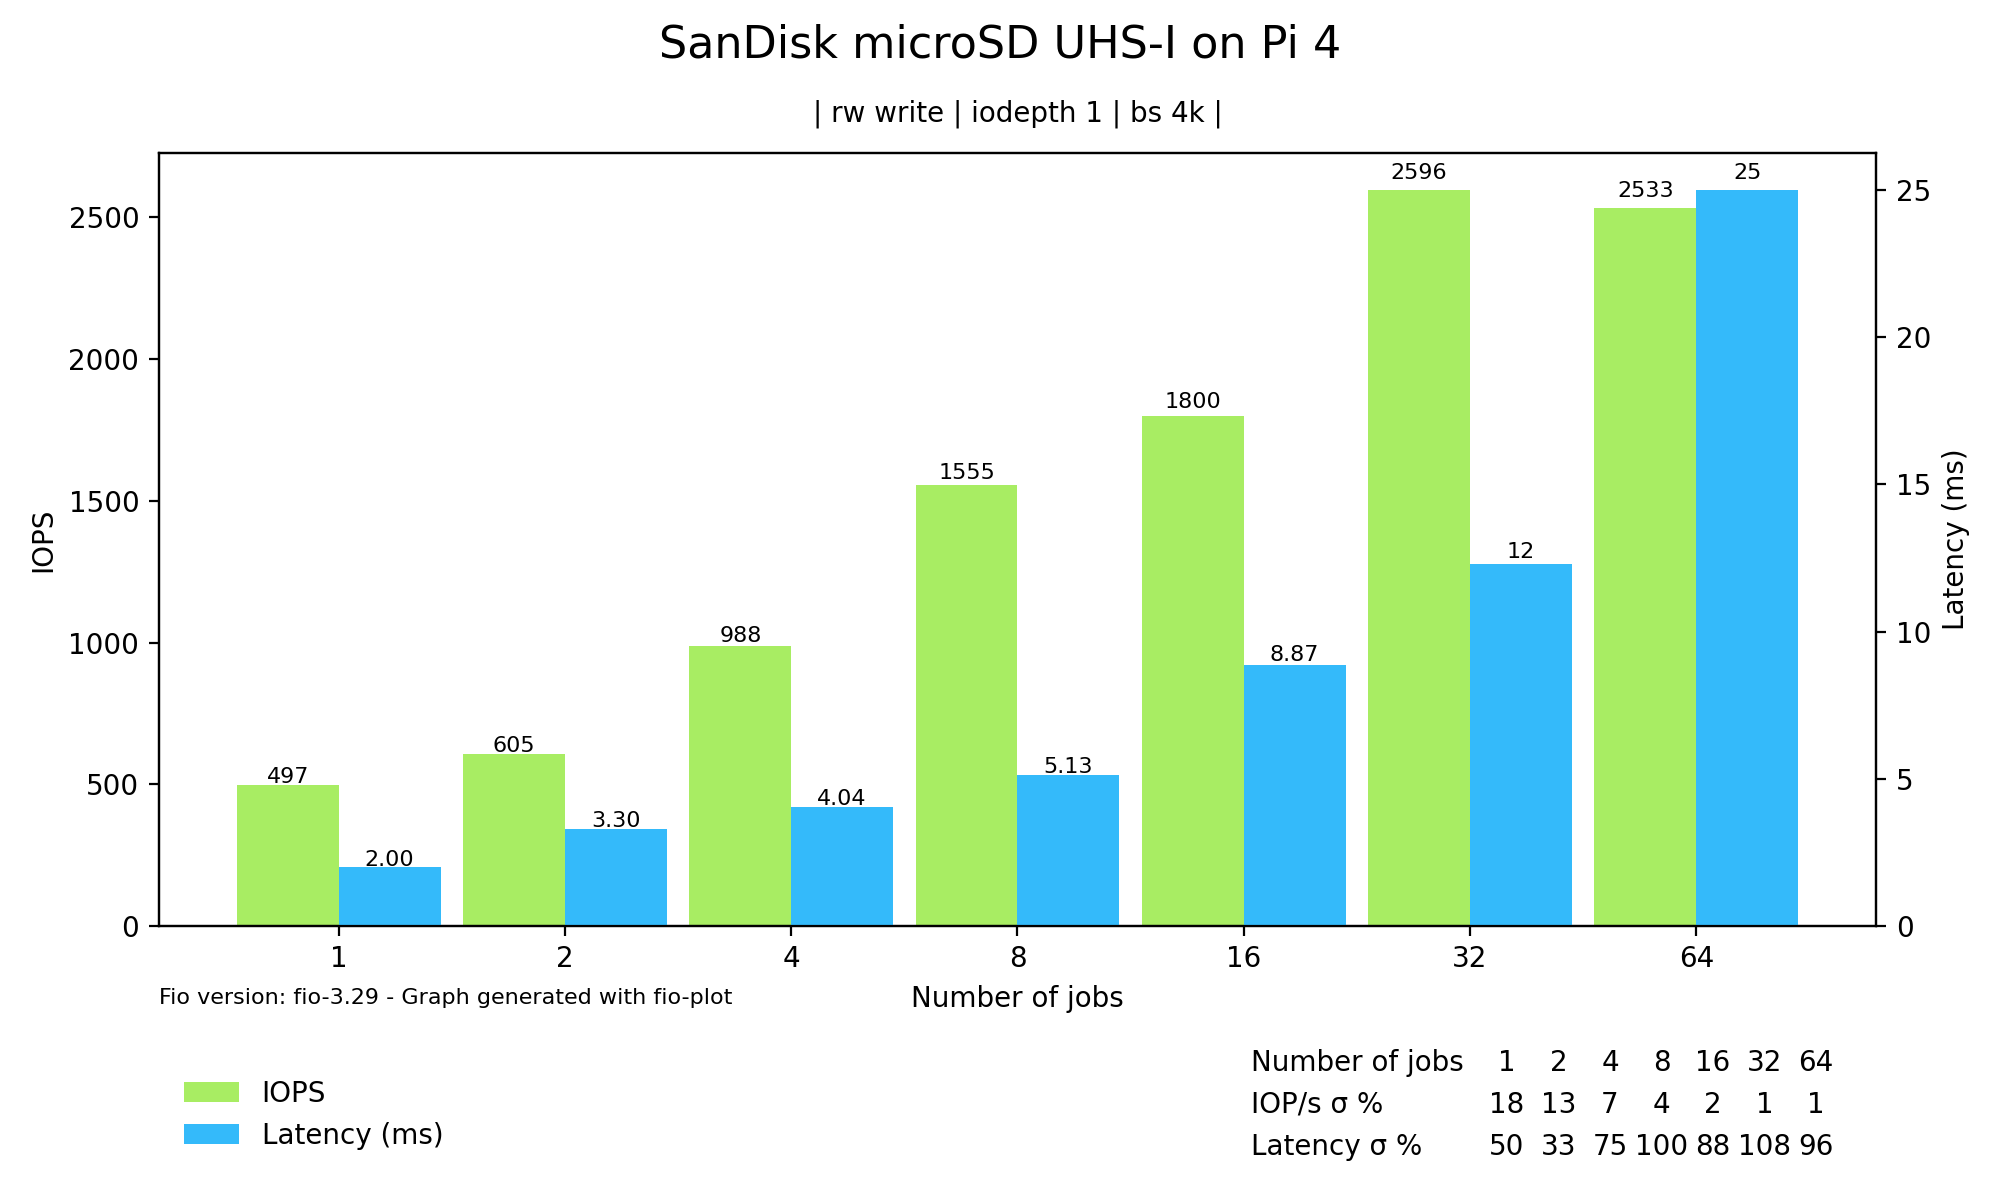
\includegraphics[width=0.8\textwidth]{images/results/sandisk-host-libaio-write-numjobs-iops-latency.png}
    \caption{Throughput and latency measurements on the host as a function of the number of concurrent processes issuing asynchronous writes.}
    \label{images:fundamentals/net-ns-veth-arch.jpg}
\end{figure}

\begin{figure}[H]
    \centering
    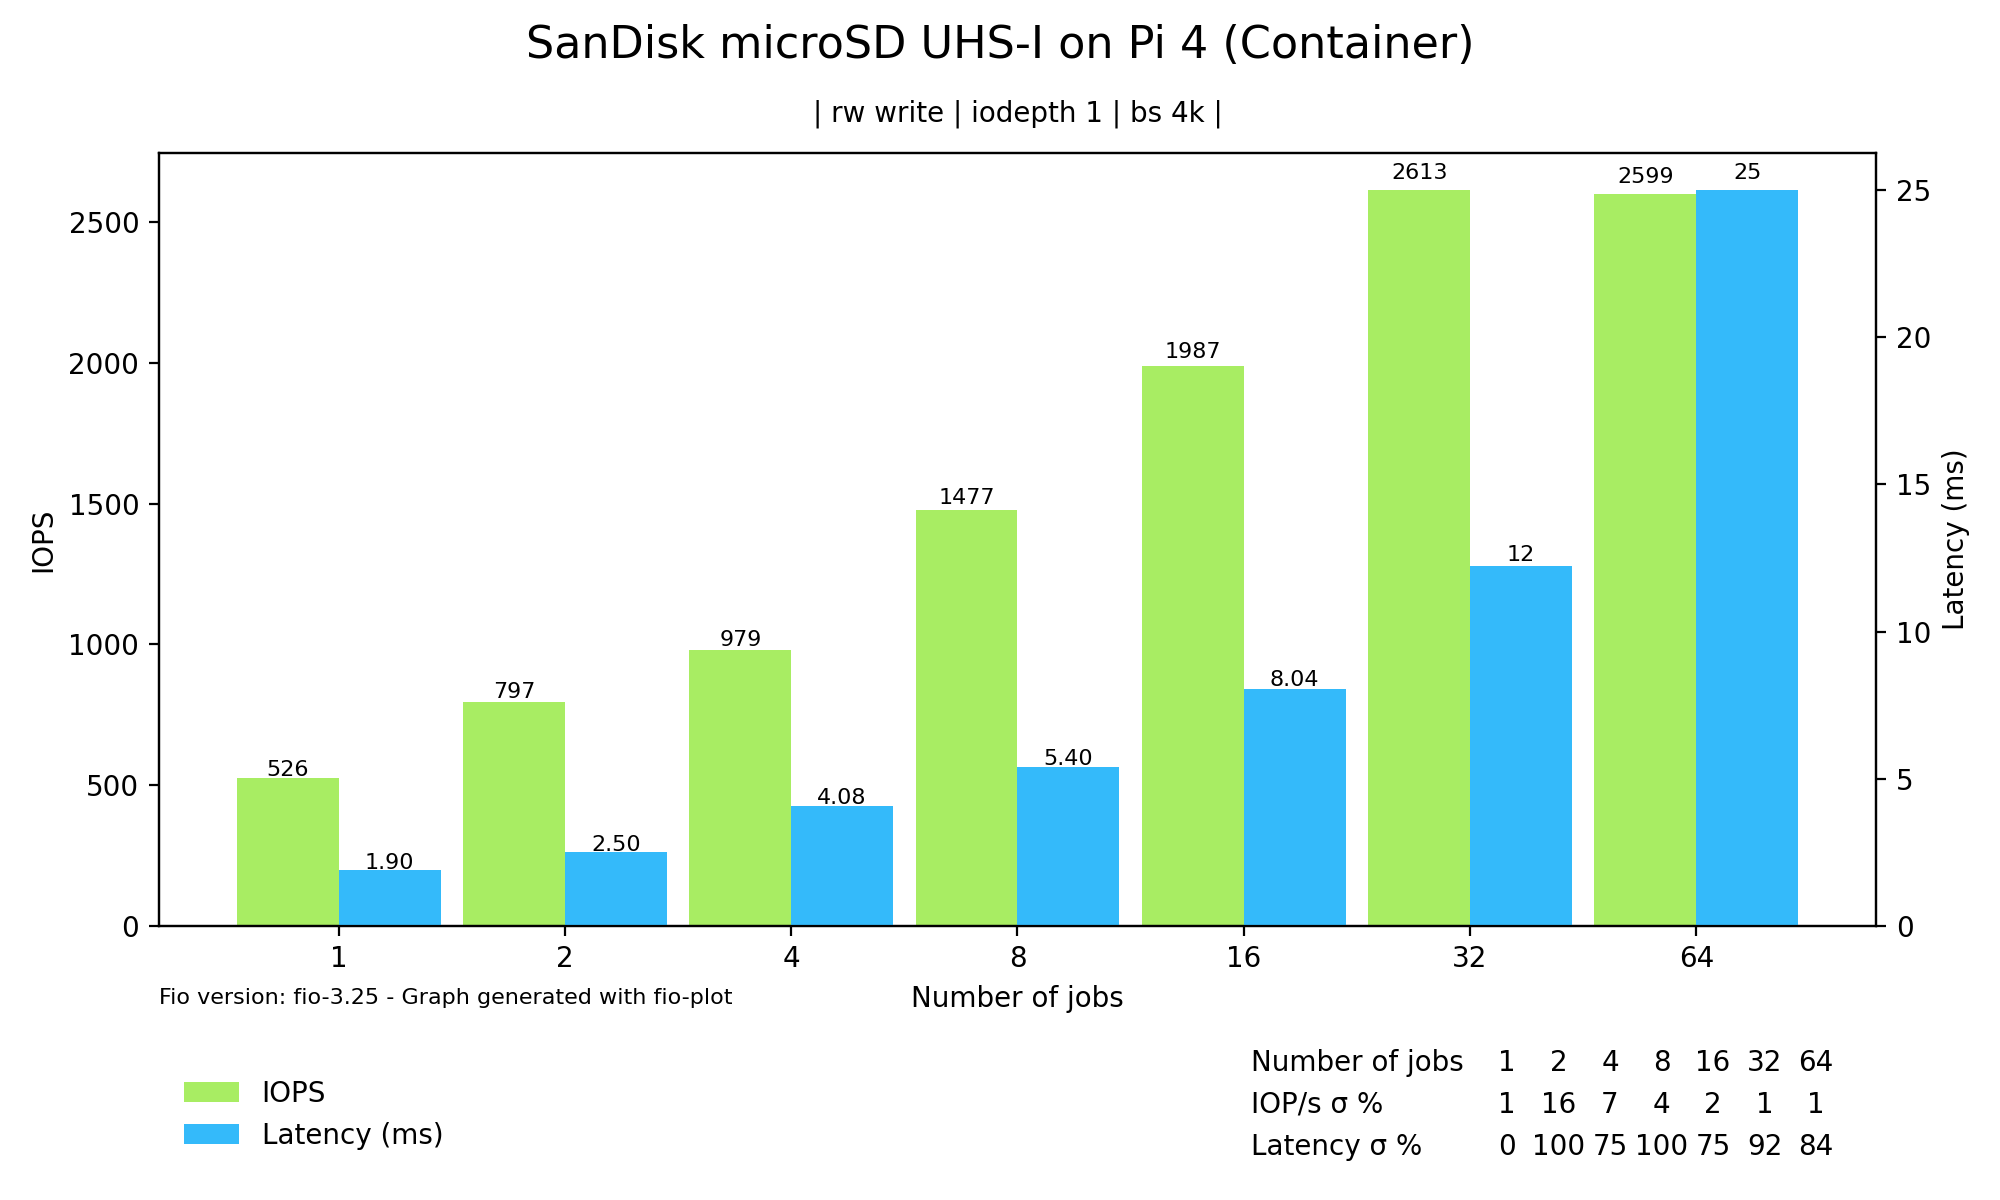
\includegraphics[width=0.8\textwidth]{images/results/sandisk-libaio-write-num-jobs-iops-latency.png}
    \caption{Asynchronous write latency and read throughput measured as a function of the number of concurrent processes inside a container}
    \label{images:fundamentals/net-ns-veth-arch.jpg}
\end{figure}

\begin{figure}[H]
    \centering
    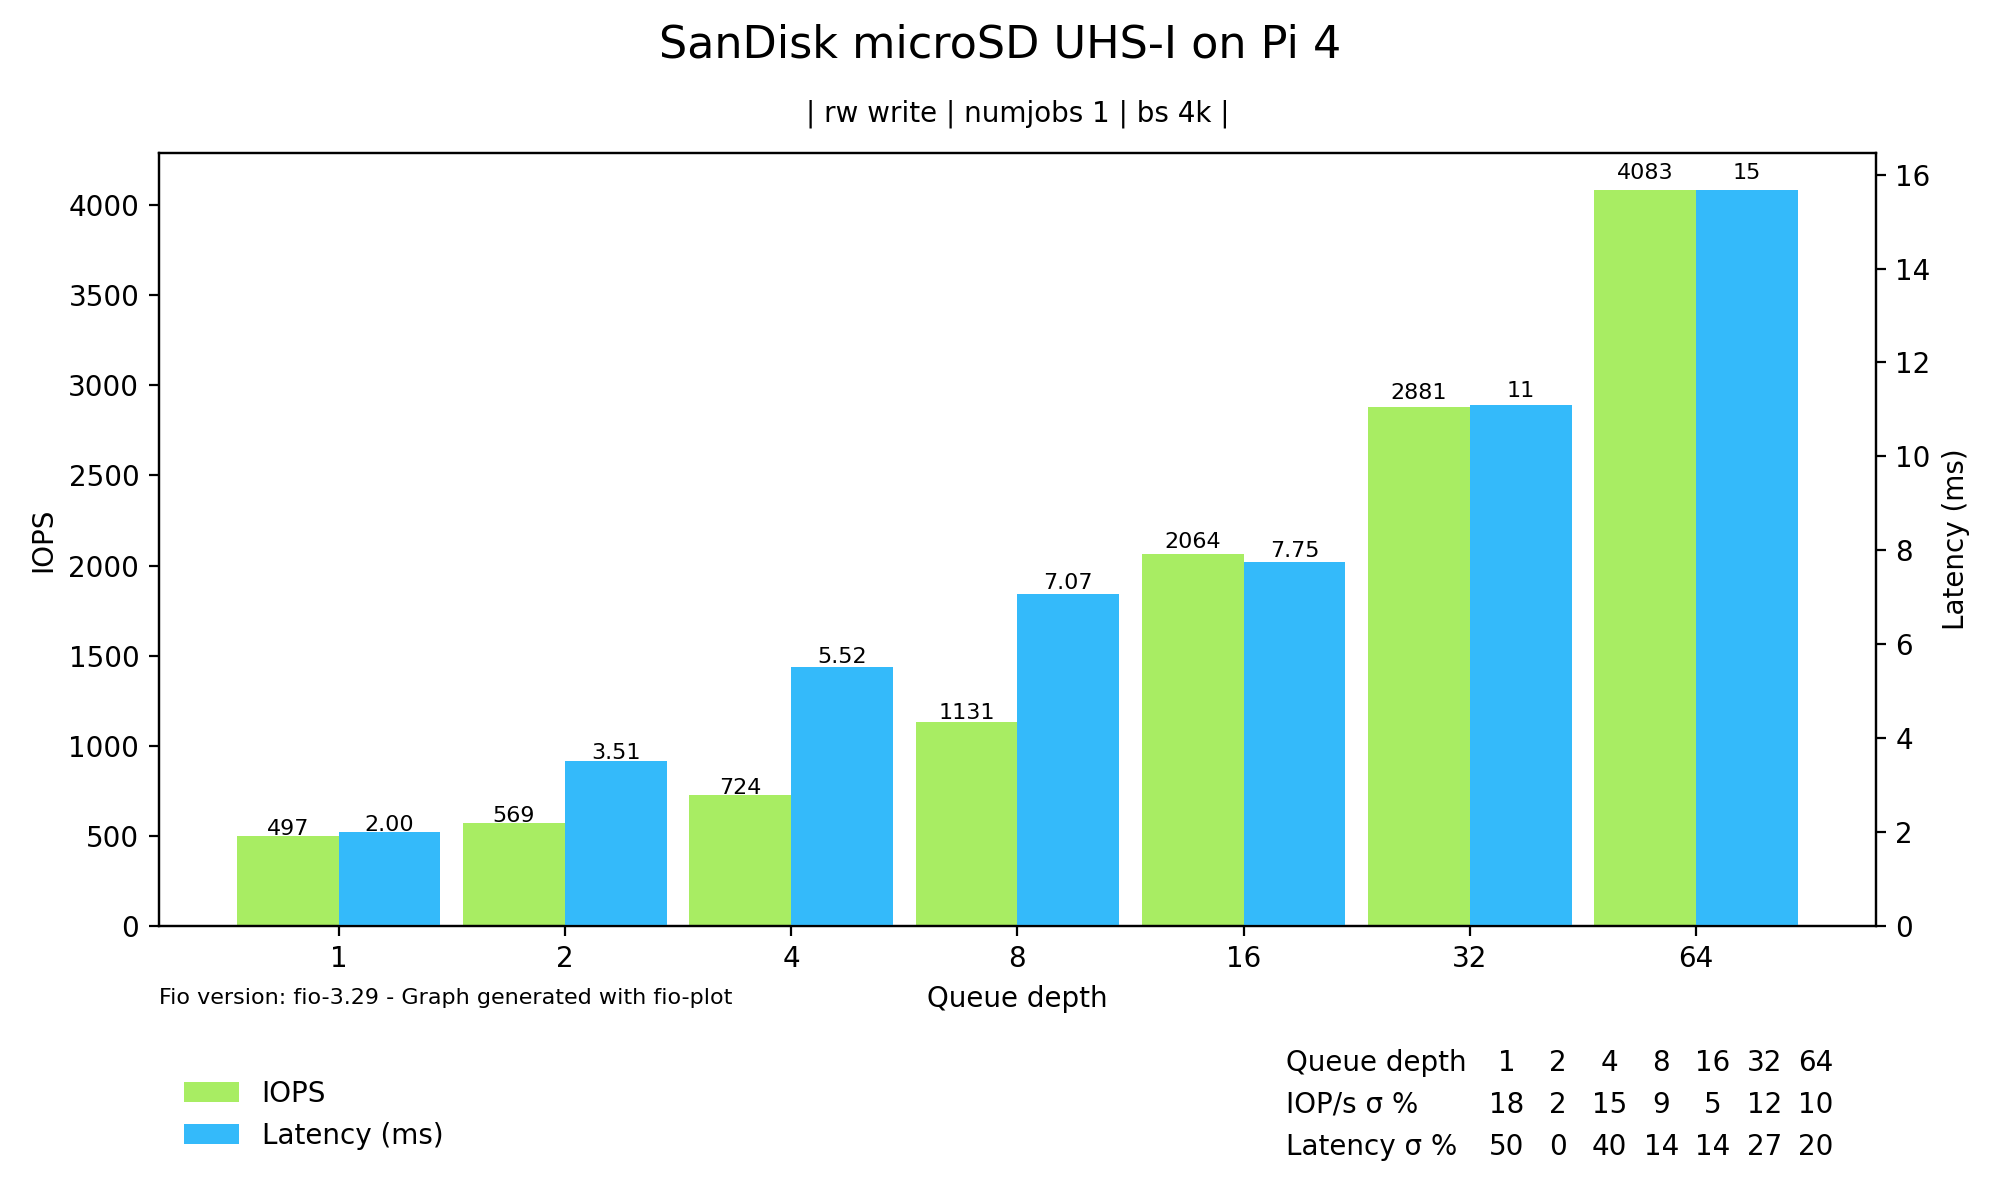
\includegraphics[width=0.8\textwidth]{images/results/sandisk-host-libaio-write-queue-depth-iops-latency.png}
    \caption{Throughput and latency measurements on the host as a function of the transmission queue length holding requests for asynchronous writes.}
    \label{images:fundamentals/net-ns-veth-arch.jpg}
\end{figure}

\begin{figure}[H]
    \centering
    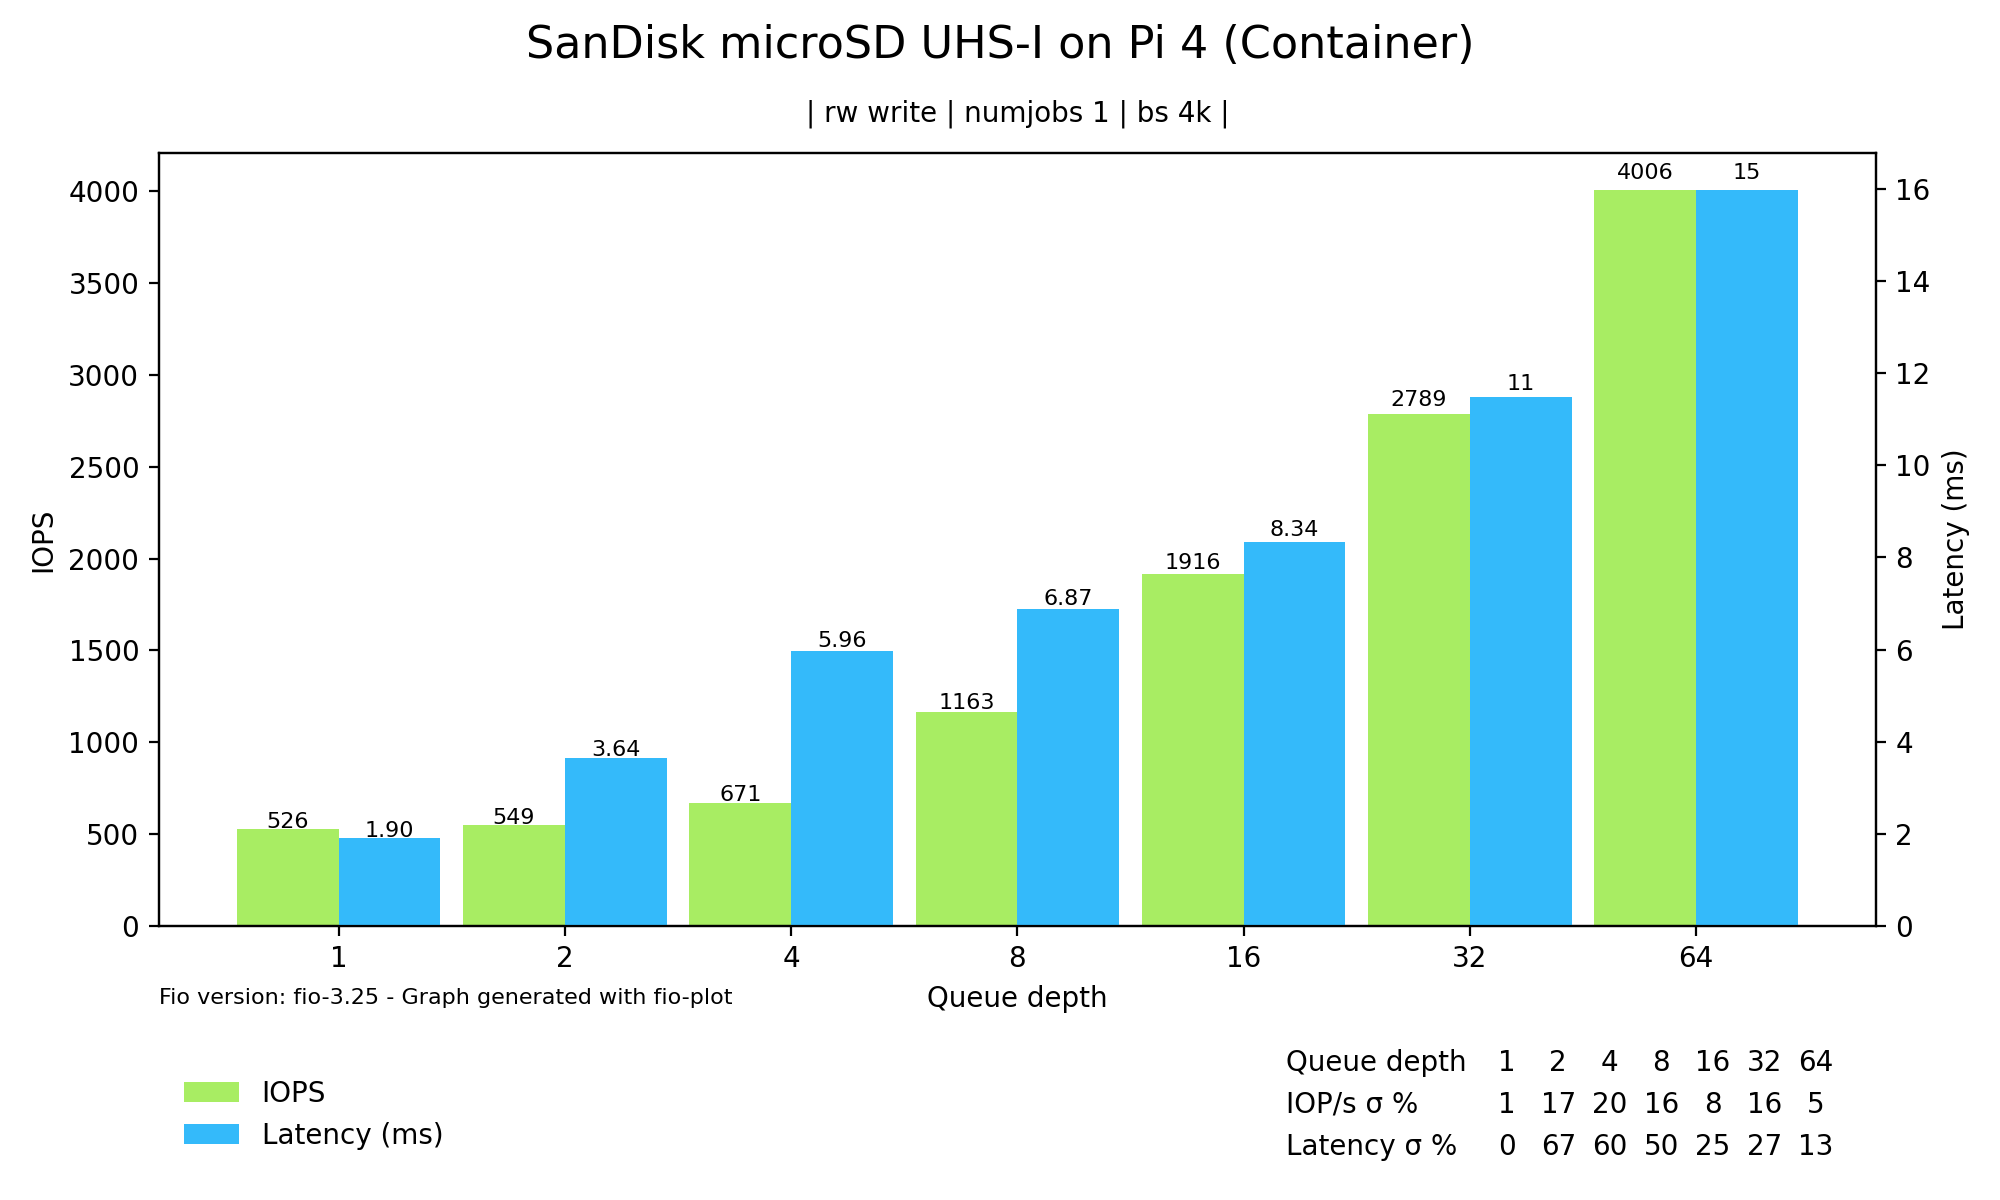
\includegraphics[width=0.8\textwidth]{images/results/sandisk-libaio-write-queue-depth-iops-latency.png}
    \caption{Throughput and latency measurements witihn a container as a function of the transmission queue length holding requests for asynchronous writes.}
    \label{images:fundamentals/net-ns-veth-arch.jpg}
\end{figure}

\begin{figure}[H]
    \centering
    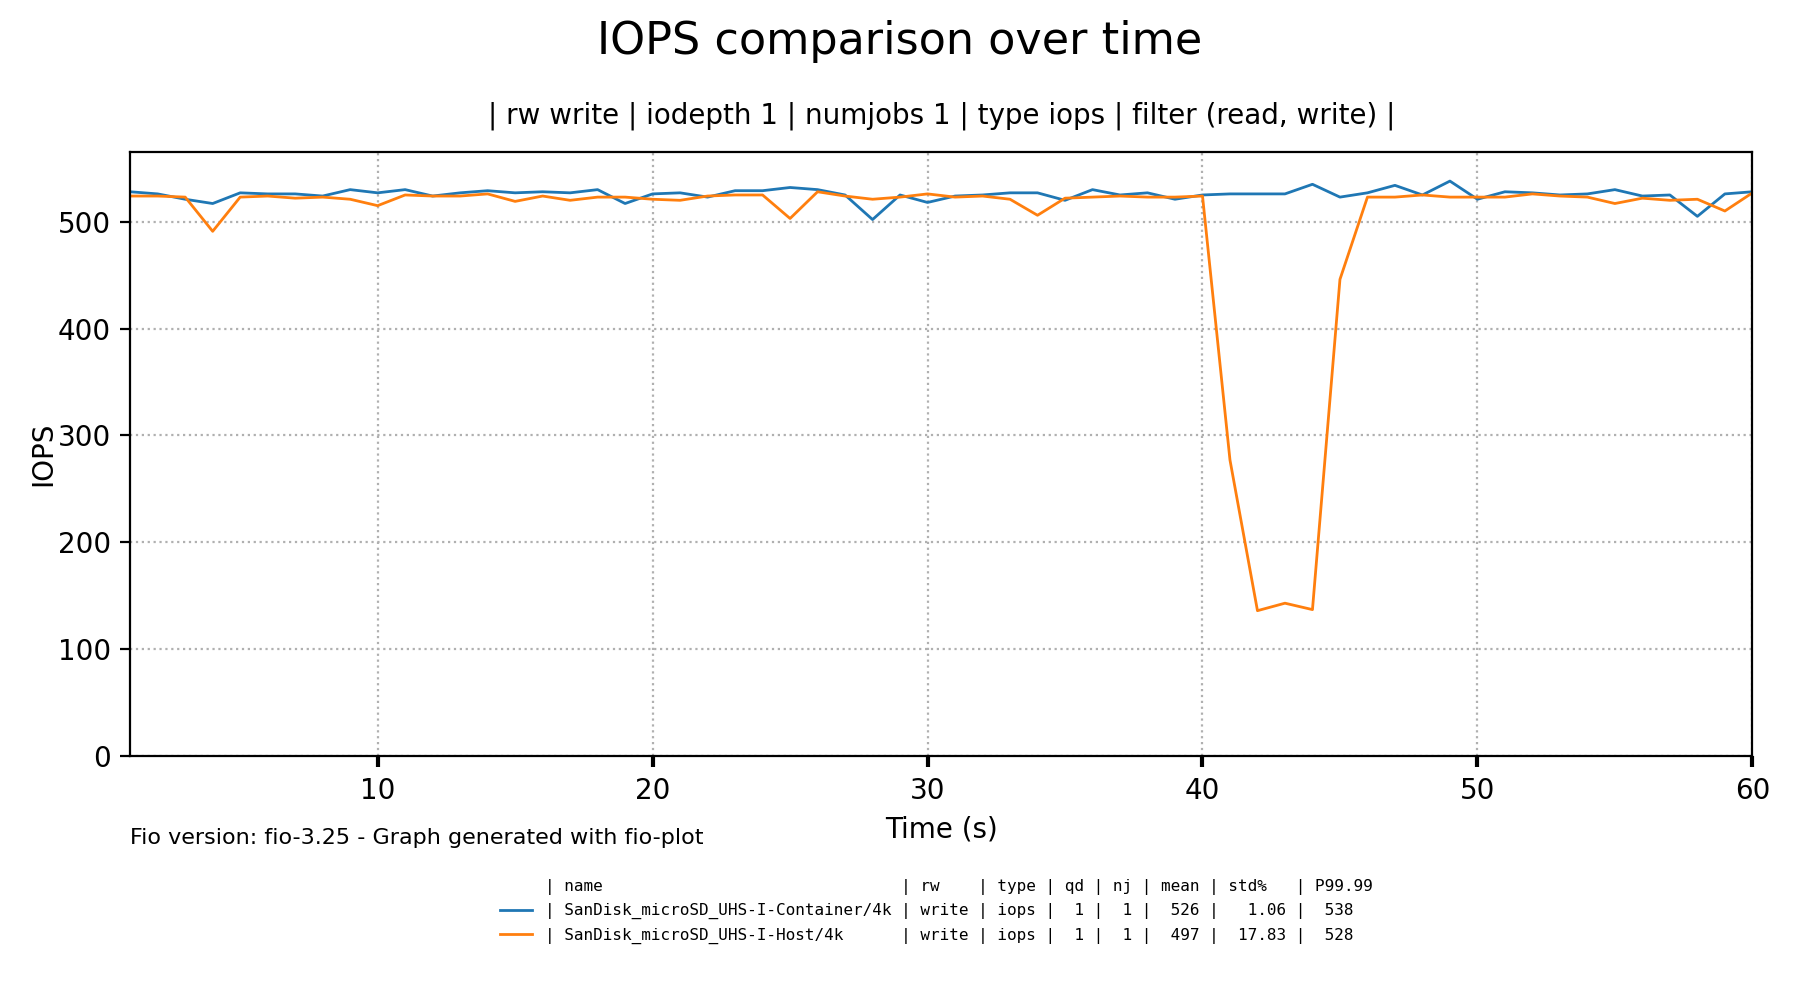
\includegraphics[width=0.8\textwidth]{images/results/sandisk-libaio-iops-write-comparison.png}
    \caption{Asynchronous write throughput on the host and inside a container, compared over time}
    \label{images:fundamentals/net-ns-veth-arch.jpg}
\end{figure}

\begin{figure}[H]
    \centering
    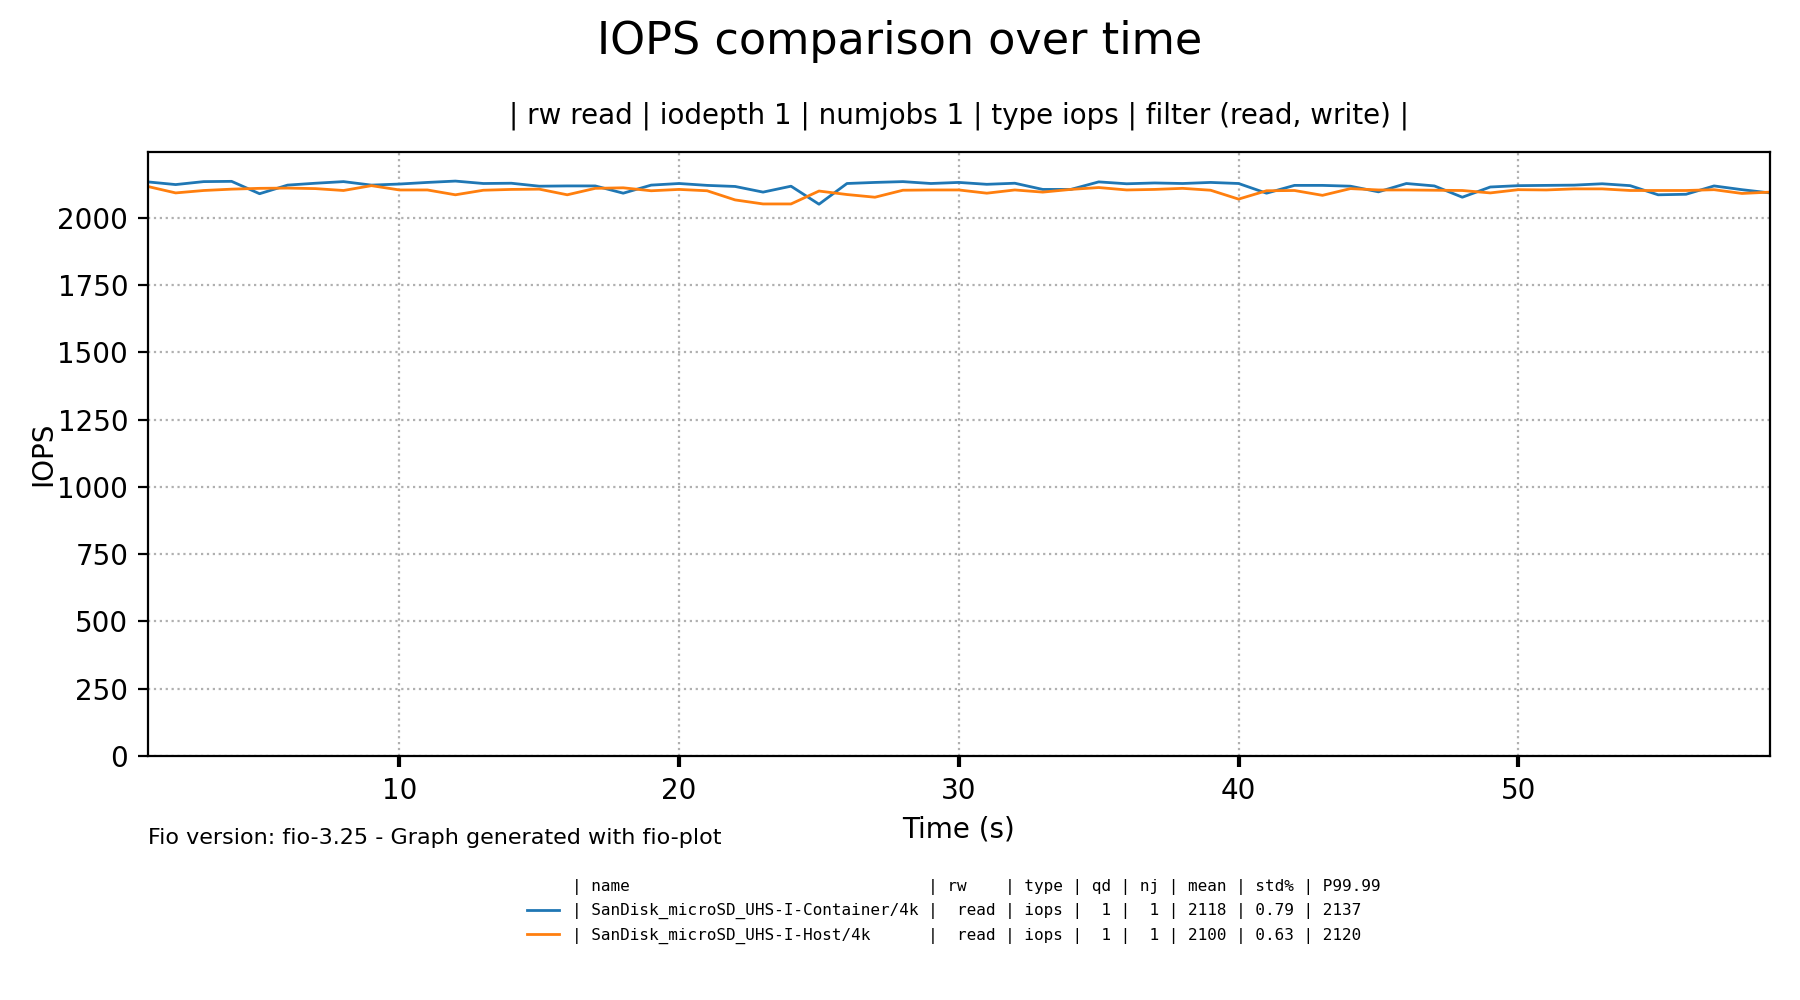
\includegraphics[width=0.8\textwidth]{images/results/sandisk-libaio-iops-read-comparison.png}
    \caption{Asynchronous read throughput on the host and inside a container, compared over time}
    \label{images:fundamentals/net-ns-veth-arch.jpg}
\end{figure}

\section{Network}
\label{ch:experiment/network}

\begin{figure}[H]
    \centering
    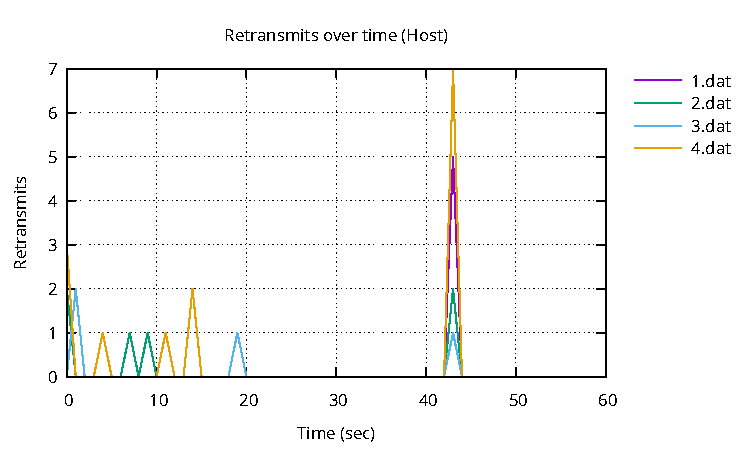
\includegraphics[width=1\textwidth]{images/results/network-host-retransmits.pdf}
    \caption{Number of packet retransmissions plotted over time on the host}
    \label{ticket-builder-class}
\end{figure}

\begin{figure}[H]
    \centering
    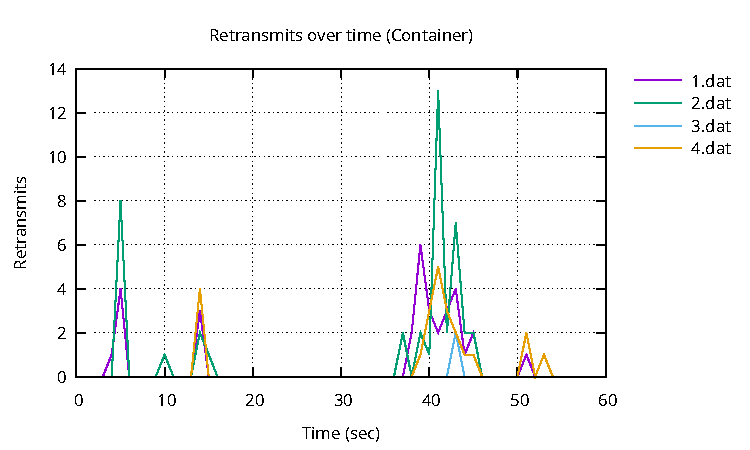
\includegraphics[width=1\textwidth]{images/results/network-retransmits-container.pdf}
    \caption{Number of packet retransmissions plotted over time within a container}
    \label{ticket-builder-class}
\end{figure}

\begin{figure}[H]
    \centering
    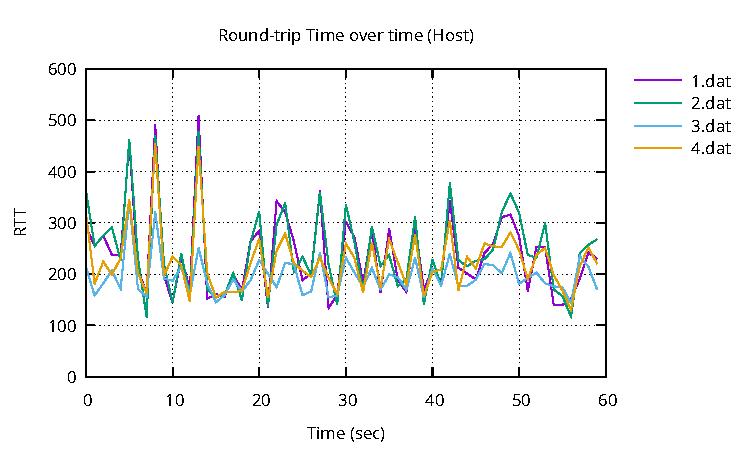
\includegraphics[width=1\textwidth]{images/results/network-host-rtt.pdf}
    \caption{Network latency (round-trip time) measured over time on the host}
    \label{ticket-builder-class}
\end{figure}

\begin{figure}[H]
    \centering
    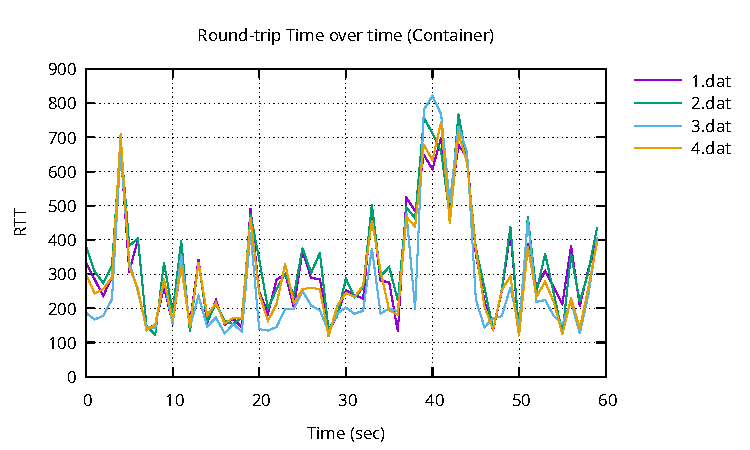
\includegraphics[width=1\textwidth]{images/results/network-rtt-container.pdf}
    \caption{Network latency (round-trip time) measured over time within a container}
    \label{ticket-builder-class}
\end{figure}

\begin{figure}[H]
    \centering
    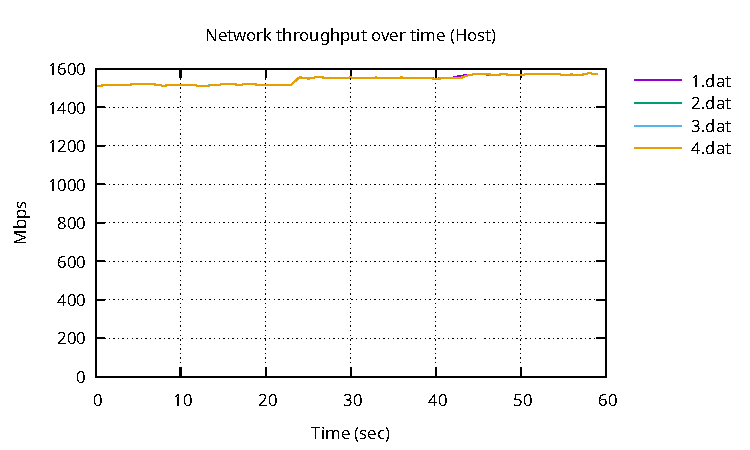
\includegraphics[width=1\textwidth]{images/results/network-host-throughput.pdf}
    \caption{Network throughput measured as megabits per second over time on the host}
    \label{ticket-builder-class}
\end{figure}

\begin{figure}[H]
    \centering
    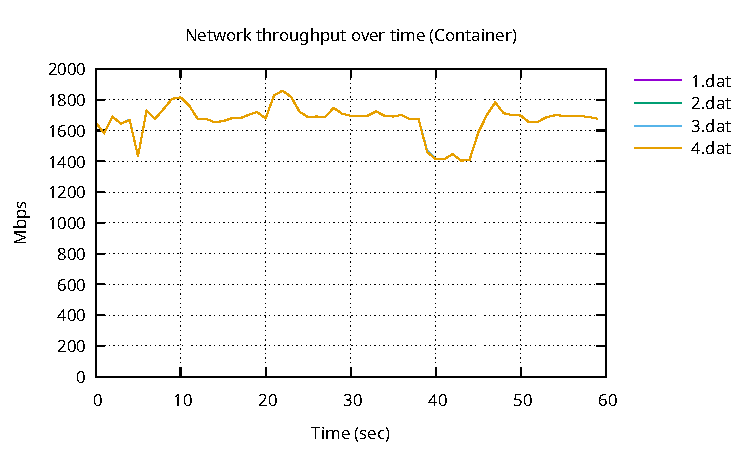
\includegraphics[width=1\textwidth]{images/results/network-throughput-container.pdf}
    \caption{Network throughput measured as megabits per second over time within a container}
    \label{ticket-builder-class}
\end{figure}